\documentclass{article} %basic LaTeX document type

%set capital Roman numeral section headings
%set capital Aramaic letters subsection headings
%set capital Arabic numbers subsubsection headings
\renewcommand\thesection{\Roman{section}.}
\renewcommand\thesubsection{\thesection\Alph{subsection}.}
\renewcommand\thesubsubsection{\thesubsection\arabic{subsubsection}.}

%set capital Roman numeral table numeration
\renewcommand*\thetable{\Roman{table}} 

%package needed for next lines
%makes section headings bold and upper case characters
%makes subsubsection headings in italics
\usepackage[explicit]{titlesec}
\titleformat{\section}{\bfseries}{\thesection}{1em}{\MakeUppercase{#1}}
\titleformat{\subsubsection}{\itshape}{\thesubsubsection}{1em}{#1}

%\linespread{2}       %option 1 for making text double-spaced
\usepackage{setspace} %option 2 for making text double-spaced
\doublespacing

%makes first paragraph of section indented (non-first are by default)
%set size of indentation (15pt is default)
\usepackage{indentfirst}
\setlength{\parindent}{25pt}

%set size of all margins
\usepackage[margin=1.3in]{geometry}
%can set margin sizes which are not the same in this way
%\usepackage[left=1in, top=1in, right=1in, bottom=1in]{geometry}

%package which returns number of last page (same as number of pages)
%package which counts the number of tables and/or figures
\usepackage{lastpage}
\usepackage[figure,table]{totalcount}

%enable `align' equation types
%enable `multirow' capability in tables
%enable figures
\usepackage{amsmath}
\usepackage{multirow}
\usepackage[dvipdfmx]{graphicx}

%enables double spaced footnotes
\usepackage[]{footmisc}

%enables subfigures
%enables subfigure captions
%sets table caption formatting options to meet NSE requirements
%sets figure caption options to meet NSE requirements
\usepackage{caption}
\usepackage[labelformat=simple]{subcaption}
\captionsetup[table]{labelsep=newline,name=TABLE}
\captionsetup[figure]{name=Fig.,labelsep=period}

%sets labeling of footnotes
%double spacing of footnotes
\renewcommand{\thefootnote}{\alph{footnote}}
\renewcommand{\footnotelayout}{\doublespacing}

%enables proper labeling of subfigures
\renewcommand*\thesubfigure{(\alph{subfigure})}

%--------------
\usepackage{paralist}	
\usepackage{amssymb}
\usepackage{epsfig}
\usepackage[mathcal]{euscript}
\usepackage{setspace}
\usepackage{color}
\usepackage{array}
\renewcommand{\ttdefault}{cmtt}
% The float package HAS to load before hyperref
\usepackage{float} % for psuedocode formatting
\usepackage{xspace}
\usepackage{mathrsfs}
\usepackage[pdftex,hidelinks]{hyperref}
\usepackage{stmaryrd} % for short right arrow
\usepackage[export]{adjustbox} % to use max height in includegraphics
\usepackage{placeins} % for float barriers

%-------------
\newcommand{\sa}{\shortrightarrow}
\newcommand{\bo}{\mathbf\Omega}
\newcommand{\vecr}{\textbf{r}}
\newcommand{\sn}{S$_\mathrm{N}$}
\newcommand{\pn}{P$_\mathrm{N}$}
\newcommand{\ve}[1]{\ensuremath{\mathbf{#1}}}
\newcommand{\Ye}[2]{\ensuremath{Y^e_{#1}(\bo_#2)}}
\newcommand{\Yo}[2]{\ensuremath{Y^o_{#1}(\bo_#2)}}
\newcommand{\Sigg}[1]{\ensuremath{\Sigma^{g'\sa g}_{\text{s},#1}}}
\newcommand{\even}{\ensuremath{\phi^g}}
\newcommand{\odd}{\ensuremath{\vartheta^g}}
\newcommand{\Gij}[2]{\sum_{\ell=0}^L\frac{2\ell+1}{4\pi}P_{\ell}(\bo_#1\cdot\bo_#2)}
\newcommand{\Sij}[2]{\Sigma^{g'\rightarrow g}_{\text{s,L}}(\bo_#1\cdot\bo_#2)}
\newcommand{\fq}{\qquad\qquad\qquad\qquad}
\newcommand{\st}{\tilde{S}}
\newcommand{\E}[1]{$\times10^{#1}$}
\newcommand{\fwc}{\mbox{FW-CADIS}}

\begin{document}

%Define fields for \maketitle  (fields are \author, \date, \thanks, and \title)

\title{Assessment of the Lagrange Discrete Ordinates Equations for
Three-Dimensional Neutron Transport} %title of paper

\author{
\vspace{20mm}
%list of authors, with corresponding author marked by asterisk
\\Kelly L.\ Rowland,$^{\text{a}}$  Cory D.\ Ahrens,$^\text{b}$ Steven Hamilton,$^\text{c}$ 
\\and R.N.\ Slaybaugh$^{\text{a},\ast}$\\[4pt] 
%affiliations of authors
\textit{$^a$University of California, Berkeley, Nuclear Engineering Department}\\[-10pt]
\textit{4173 Etcheverry Hall, Berkeley, CA 94720, USA} \\[-5pt]
\textit{$^b$X Theoretical Design Division, Primary Physics Group}\\[-10pt]
\textit{Los Alamos National Laboratory, Los Alamos, NM 87545, USA}\\[-5pt]
\textit{$^c$Oak Ridge National Laboratory, Radiation Transport and Criticality Group} \\ [-10pt]
\textit{P.O. Box 2008, Oak Ridge, TN 37831-6170, USA} \\ [-2pt]
{$^\ast$slaybaugh@berkeley.edu}} %address and email address for correspondence

% instead of returning the date, this repurposes the \maketitle command to 
% print the number of pages, tables, and figures
\date{
\vspace{40mm}
Number of pages: \pageref{LastPage} \\  
Number of tables: \totaltables \\
Number of figures: \totalfigures \\}                                              

\maketitle

\pagebreak

\begin{abstract}
{
The Lagrange Discrete Ordinates (LDO) equations, developed by Ahrens as an
alternative to the traditional discrete ordinates formulation, have been
implemented in Denovo, a three-dimensional radiation transport code developed
by Oak Ridge National Laboratory. The LDO equations retain the formal structure
of the classical discrete ordinates equations but treat particle scattering
in a different way. Solutions of the LDO equations have an interpolatory
structure such that the angular flux can be naturally evaluated at directions
other than the discrete ordinates used in arriving at the solutions, and the
ordinates themselves may be chosen in a strategic way for the problem
under consideration. Of particular interest is that the LDO equations have been
shown to mitigate ray effects at increased angular resolutions. In this paper
we present scalar flux solutions of the LDO equations for a small
number of test cases of interest and compare the results against flux solutions
generated using standard quadrature types. The LDO equations' flux solutions
were found to be comparable to those resultant from the standard quadrature
types in value; results from the LDO equations were also found to be
commensurate with those of standard quadrature types when comparing the flux
solutions in the context of the experimental benchmark test case examined.

Keywords: quadrature; Lagrange; discrete ordinates; transport
}
\end{abstract}

\pagebreak

%%---------------------------------------------------------------------------%%
\section{Introduction}
\label{sec:intro}

With the recent rise in high-performance computing, large-scale  three-
dimensional neutral particle transport is becoming increasingly commonplace.
One common solution approach is to discretize all of the independent variables
of the steady-state Boltzmann transport equation and solve the resultant
systems of equations deterministically. The classic discrete ordinates (\sn)
method is well-known and frequently used in deterministic transport, but it
can suffer from inaccuracies in scalar particle flux solutions brought about
by angular discretization (termed ``ray effects'').

The Lagrange Discrete Ordinates (LDO) equations, developed by Ahrens
\cite{ahrens}, are formally equivalent to the classic \sn\ equations; they
retain the formal structure of the classical discrete ordinates equations but
treat particle scattering in a different way. Solutions of the LDO equations
have an interpolatory structure such that the angular flux can be naturally
evaluated at directions other than the discrete ordinates used in arriving at
the solutions, providing a high degree of flexibility. Furthermore, the
ordinates themselves may be chosen in a strategic way for the problem under
consideration.

Fundamental studies of the LDO formulation were conducted in their development
which showed that the LDO equations mitigate ray effects at increased angular
resolutions. However, the equations have never before been implemented in a
full-scale radiation transport framework. In this paper we will explore and
assess deterministic scalar flux solutions from the LDO equations for real
problems in production-level software.

Studies performed in this work compare scalar flux solutions from the LDO
equations with those from quadruple range (QR), Galerkin, and linear-
discontinuous finite element (LDFE) quadrature sets. Three relevant test case
scenarios are examined to provide a small array of results of interest to the
community; we test both neutron and photon transport. The LDO equations'
scalar flux solutions were found to be consistent with those of the standard
quadrature types for all three test case scenarios and commensurate with
those of the standard quadrature types when comparing the flux solutions in
the context of the experimental benchmark test case examined. The
demonstration of the accuracy of the LDO equations in a full-scale transport
code opens the door to their strategic use for problems containing strong
angular anisotropies or in which specific directions are of particular
interest.

The remainder of the paper is structured as follows: background information
regarding the main components of this work is given, followed by descriptions
of the test case scenarios employed and the choices made in parameter selection
for the calculations performed. Numerical results are presented and discussed
and we close the paper with concluding remarks and suggestions for future work.

%%---------------------------------------------------------------------------%%
\section{Background}
\label{sec:background}

We start by giving background information on constituent components of this
work. Primarily, we will briefly cover the traditional discrete ordinates
(\sn) approximation. Then, we give a short introduction to the Lagrange
Discrete Ordinates (LDO) equations. As one of the points of interest in the
LDO equations is their unique handling of angular discretization and particle
scattering, we will focus discussions in such a way as to highlight the
actualities and implications of this difference. We implemented this work in
Denovo, a three-dimensional discrete ordinates radiation transport code
developed by Oak Ridge National Laboratory \cite{denovo}. Denovo is part of
the Exnihilo framework that allows for multiple combinations of spatial
discretizations, quadrature sets, and solution methods.

%%---------------------------------------------------------------------------%%
\subsection{Classical Discrete Ordinates Equations}

The steady-state Boltzmann transport equation is

\begin{multline}
\bo \cdot \nabla \psi(\vecr,E,\bo) + \Sigma_t(\vecr,E) \psi(\vecr,E,\bo) = \\
\int_0^\infty\int_{4\pi} \Sigma_s(\vecr,E'\rightarrow E,\bo'\cdot\bo)
\psi(\vecr,E',\bo')d\bo'dE' + Q(\vecr,E,\bo),
\label{eq:bte}
\end{multline}

\noindent where $\psi$ denotes the angular flux, $\vecr$ is the particle
position, $E$ is the energy of the particle,
and $\bo$ is the unit vector of direction of travel of the particle. As it is
pertinent to the material presented here, we will briefly note the discrete
ordinates method employed for angular discretization; full detail may
be found in Reference \cite{denovo}.

The \sn\ approximation is

\begin{multline}
\bo_n \cdot \nabla \psi_n^g(\vecr) + \Sigma_t^g(\vecr)\psi_n^g(\vecr) = \\
\sum_{g'=0}^{G-1}\sum_{\ell=0}^{P}\Sigma_{s,\ell}^{g'\sa g}(\vecr)
\bigg[\Ye{\ell 0}{n}\phi_{\ell 0}^{g'}(\vecr) + \sum_{m=1}^{\ell}
\bigg(\Ye{\ell m}{n}\phi_{\ell m}^{g'}(\vecr) \\
 + \Yo{\ell m}{n}\vartheta_{\ell m}^{g'}(\vecr)\bigg)\bigg]
+ Q_n^g(\vecr),
\label{eq:sn}
\end{multline}

\noindent where a standard multigroup energy approximation is used ($G$ is the
number of discrete energy groups corresponding to the discretization index
$g$) and the  upper limit of summation for the scattering term spherical
harmonic expansion, denoted as $P$ in Equation \ref{eq:sn}, is known as the
``\pn\ order''. The angles are integrated by a quadrature rule with $N$
ordinates such that

\begin{equation}
\int_{4\pi} d\bo = \sum_{n=1}^{N}w_n = 4\pi.
\label{eq:quadrule}
\end{equation}

\noindent The scattering source is expanded in terms of spherical harmonics:

\begin{equation}
\phi_{\ell,i,j,k}^{g}=\sum_{n=1}^N \Ye{\ell m}{n}w_n\psi^{g,n}_{i,j,k}\ \text{ and }\
\vartheta_{\ell,i,j,k}^{g} = \sum_{n=1}^N \Yo{\ell m}{n}w_n\psi^{g,n}_{i,j,k},
\label{sph_harm_exp}
\end{equation}

\noindent where $\phi$ and $\vartheta$ are referred to as the ``angular flux
moments''. Here, $\Ye{\ell m}{n}$ and $\Yo{\ell m}{n}$ are the ``even'' and
``odd'' real components of the spherical harmonic functions, defined as
\cite{exmm}

\begin{equation}
\Ye{\ell m}{n} = (-1)^m\sqrt{(2-\delta_{m0})\frac{2\ell+1}{4\pi}
                       \frac{(\ell-m)!}{(\ell+m)!}}
                       P_{\ell m}(\cos\theta)\cos(m\varphi),
\label{eq:sph_e}
\end{equation}
\begin{equation}
\Yo{\ell m}{n} = (-1)^m\sqrt{(2-\delta_{m0})\frac{2\ell+1}{4\pi}
                       \frac{(\ell-m)!}{(\ell+m)!}}
                       P_{\ell m}(\cos\theta)\sin(m\varphi).
\label{eq:sph_o}
\end{equation}

\noindent In Equations \ref{eq:sph_e} and \ref{eq:sph_o},
$P_{\ell m}(\cos\theta)$ is the associated Legendre polynomial and
$(\theta,\varphi)$ are the components of $\bo$.

%%---------------------------------------------------------------------------%%
\subsection{Lagrange Discrete Ordinates (LDO) Equations}

The Lagrange Discrete Ordinates (LDO) equations are formally the same as the
traditional \sn\ equations but feature several distinct and important
differences. From the derivation in Reference \cite{ahrens}, the equations,
without energy discretization, are written as

\begin{multline}
\bo_n\cdot\nabla\psi_{n}(\vecr,E) + 
\Sigma_{t}(\vecr,E)\psi_{n}(\vecr,E) = \\
\int_0^\infty\sum_{m=1}^{N}\sum_{n'=1}^{N}\langle L_{n'},L_{m}\rangle
\Sigma_{s,L}(\vecr,E'\rightarrow E)(\bo_{m}\cdot\bo_n)\psi_{n'}(E')dE'
+ Q_{n}(E),
\end{multline}

\noindent where $N$ is the number of discrete angles used in the formulation
and is a property of the maximum degree of integration of the quadrature set
on which the equations are based, $L_n$ is the $n^{th}$ Lagrange function, and
$\Sigma_{s,L}$ is the scattering cross section restricted to maximum degree
$L$.

The notable differences between the LDO equations and the classical \sn\
equations can be summarized as:

\begin{enumerate}
\item{The LDO solution has an interpolatory structure in angle, which allows
      the angular flux to naturally be evaluated at directions other than those
      in the quadrature set used to construct the equations.}
\item{The LDO formulation does not require calculation of spherical harmonic
      moments.}
\item{The positive-weight quadrature sets on which the LDO equations are based
      can integrate spherical harmonics ranging from degree 0 to degree 165.}
\end{enumerate}

For a given fixed maximum degree of integration $L$, the corresponding number
of ordinates in the LDO formulation is $(L+1)^2$. The LDO equations are
developed with and must be evaluated at a fundamental system of points for the
subspace of spherical harmonics. Ahrens provides references for examples of
construction methods of these point systems \cite{ahrens}. Like Ahrens, we
have chosen to use the extremal point sets developed and distributed by
Womersley \cite{wom}.

%%---------------------------------------------------------------------------%%
\section{Methodology}

First, a comparison of the traditional formulation of the discrete ordinates
equations with the LDO equations is presented to demonstrate the difference
in implementing the two separate sets of equations. Then, a brief discussion
of  scattering is given to highlight the specific differences between the two
sets of equations with respect to what scattering data is needed and how
scattering is handled from the perspective of implementation.

%%---------------------------------------------------------------------------%%
\subsection{Operator Form}
\subsubsection{Traditional Discrete Ordinates Formulation}

When considering deterministic methods, it is often instructive to think about
the transport equation in operator form. The 
operator form of the traditional discrete ordinates equations is

\begin{align}
\ve{L}\Psi &= \ve{MS}\Phi + Q, \\
\Phi &= \ve{D}\Psi\: \text{ where } \ve{D} = \ve{M}^\top\ve{W}, \\
\left(\ve{I} - \ve{DL}^{-1}\ve{MS}\right)\Phi &= \ve{DL}^{-1}Q.
\label{l_inv}
\end{align}

\noindent The operators will be defined below, with the exception of $\ve{L}$,
the transport operator. When solving Equation \ref{l_inv}, the operation
$\ve{L}^{-1}$ is referred to as a ``sweep''; $\ve{L}$ is implicitly formed as a
lower-left triangular matrix and is inverted by ``sweeping'' through the
spatial mesh in the direction of particle flow \cite{exmm}.
With this formulation, at each spatial unknown, with discrete energy groups
defined over the range $g\in[0,G-1]$, we can write

\begin{align}
    \ve{L}
    &\begin{pmatrix}
      \Psi_0 \\
      \Psi_1 \\
      \vdots   \\
      \Psi_{G-1}  \nonumber
    \end{pmatrix} = \\
    &\qquad\begin{pmatrix}
      [\ve{M}] & 0 & 0 & 0 \\
      0 & [\ve{M}] & 0 & 0 \\
      0 & 0 & \ddots & \vdots \\
      0 & 0 & \cdots & [\ve{M}] \\
    \end{pmatrix}
    %%
    \begin{pmatrix}
      [\ve{S}]_{0\sa0} & [\ve{S}]_{1\sa0} & \cdots & [\ve{S}]_{G-1\sa0} \\
      [\ve{S}]_{0\sa1} & [\ve{S}]_{1\sa1} & \cdots & [\ve{S}]_{G-1\sa1} \\
      \vdots & \vdots & \ddots & \vdots \\
      [\ve{S}]_{0\sa G-1} & [\ve{S}]_{1\sa G-1} & \cdots & [\ve{S}]_{G-1\sa G-1}
    \end{pmatrix}
    \begin{pmatrix}
      \Phi_0 \\
      \Phi_1 \\
      \vdots   \\
      \Phi_{G-1}
    \end{pmatrix}
    %%
    \\&\fq\fq\fq\qquad\qquad\qquad+
    \begin{pmatrix}
      Q_0 \\
      Q_1 \\
      \vdots  \\
      Q_{G-1}
    \end{pmatrix}, \nonumber
    \label{eq:matrix-transport}
\end{align}

\noindent where the notation $[\cdot]_g$ indicates a block matrix over all
unknowns for a single group.  

Here, the angular flux vector for group $g$ over angles $1,\ldots,N$ is defined
as

\begin{equation}
  \Psi_g = \begin{pmatrix}
    \psi^g_1 & \psi^g_2 & \psi^g_3 & \cdots \psi^g_N
  \end{pmatrix}^\top,
\label{psiv}
\end{equation}

\noindent with the external source vector $Q_g$ defined similarly. The operator
$\ve{M}$ is the ``moment-to-discrete'' matrix
used to project harmonic moments onto discrete angle space and is defined as

\begin{equation}
[\ve{M}] = \begin{pmatrix}
\Ye{00}{1} & \Ye{10}{1} & \Yo{11}{1} & \Ye{11}{1} & \cdots & \Yo{PP}{1} & \Ye{PP}{1} \\
\Ye{00}{2} & \Ye{10}{2} & \Yo{11}{2} & \Ye{11}{2} & \cdots & \Yo{PP}{2} & \Ye{PP}{2} \\
\Ye{00}{3} & \Ye{10}{3} & \Yo{11}{3} & \Ye{11}{3} & \cdots & \Yo{PP}{3} & \Ye{PP}{3} \\
\vdots     & \vdots     & \vdots     & \vdots     & \ddots & \vdots     & \vdots     \\
\Ye{00}{N} & \Ye{10}{N} & \Yo{11}{N} & \Ye{11}{N} & \cdots & \Yo{PP}{N} & \Ye{PP}{N}
  \end{pmatrix}\:.
\label{mtod}
\end{equation}

\noindent Note that $[\ve{M}]$ is dependent only on angle and is therefore the
same for each energy group. Recall that in Equation \ref{mtod}, $P$ is the \pn\
order. The operator $\ve{D}$ is the ``discrete-to-moment''
matrix; it is used to calculate the moments of the angular flux from discrete
angular flux values. $\ve{D}$ is calculated as $\ve{M}^\top\ve{W}$, where
$\ve{W}$ is a diagonal matrix of quadrature weights \cite{exmm}, and $[\ve{D}]$ is
written as

\begin{equation}
  [\ve{D}] = \begin{pmatrix}
    w_1\Ye{00}{1} & w_2\Ye{00}{2} & w_3\Ye{00}{3} & \cdots & w_N\Ye{00}{N} \\ 
    w_1\Ye{10}{1} & w_2\Ye{10}{2} & w_3\Ye{10}{3} & \cdots & w_N\Ye{10}{N} \\
    w_1\Yo{11}{1} & w_2\Yo{11}{2} & w_3\Yo{11}{3} & \cdots & w_N\Yo{11}{N} \\
    w_1\Ye{11}{1} & w_2\Ye{11}{2} & w_3\Ye{11}{3} & \cdots & w_N\Ye{11}{N} \\
    \vdots        & \vdots        & \vdots        & \ddots & \vdots        \\
    w_1\Yo{PP}{1} & w_2\Yo{PP}{2} & w_3\Yo{PP}{3} & \cdots & w_N\Yo{PP}{N} \\
    w_1\Ye{PP}{1} & w_2\Ye{PP}{2} & w_3\Ye{PP}{3} & \cdots & w_N\Ye{PP}{N}
  \end{pmatrix}\:.
\end{equation}

\noindent Like $[\ve{M}]$, $[\ve{D}]$ is dependent only on angle and is the
same for each energy group. The scattering cross section matrices are defined
as

\begin{equation}
  [\ve{S}]_{g'\rightarrow g} = \begin{pmatrix}
    \Sigg{0} & 0 & 0 & 0 & 0 & 0 & 0 \\
    0 & \Sigg{1} & 0 & 0 & 0 & 0 & 0 \\
    0 & 0 & \Sigg{1} & 0 & 0 & 0 & 0 \\
    0 & 0 & 0 & \Sigg{1} & 0 & 0 & 0 \\
    0 & 0 & 0 & 0 & \ddots   & 0 & 0 \\
    0 & 0 & 0 & 0 & 0 & \Sigg{P} & 0 \\
    0 & 0 & 0 & 0 & 0 & 0 & \Sigg{P}
  \end{pmatrix}\:.
\label{denovo_scatter}
\end{equation}

\noindent Finally, the flux moment vectors are defined as

\begin{align}
  \Phi_g = \begin{pmatrix}
    \even_{00} & \even_{10} & \odd_{11} & \even_{11} & \even_{20}
    & \cdots & \odd_{PP} & \even_{PP}
  \end{pmatrix}^\top\:.
\end{align}

\noindent As we will describe below in Section \ref{sec:flux}, the 
goal of solving the discrete ordinates equations is to solve for these flux
moments and then use the flux moments to calculate the scalar flux. In summary,
the traditional discrete ordinates discretizations are captured in the
preceding matrices; they can be used to analyze behavior and performance and
can be compared against other discretizations.

%%---------------------------------------------------------------------------%%
\subsubsection{LDO Formulation}

Although the LDO equations are formally the same as the traditional \sn\
equations, there are several key differences between the sets of equations.
Here we present and discuss the operator form of the LDO equations and
compare them to the operator form of the discrete ordinates
equations shown above. The operator form of the LDO equations is

\begin{align}
\ve{L}\Psi &= \ve{\tilde{S}J}\Psi + Q, \\
\left(\ve{I} - \ve{L^{-1} \tilde{S}J}\right)\Psi &= \ve{L^{-1}}Q.
\end{align}

\noindent Letting $\ve{D} \equiv \ve{I}$ with 
$\ve{L^{-1}} = \ve{I}\ve{L^{-1}} = \ve{D}\ve{L^{-1}}$, we then have

\begin{equation}
\left(\ve{I} - \ve{D L^{-1} \tilde{S}J}\right)\Psi = \ve{D L^{-1}}Q.
\label{ldo_op}
\end{equation}

\noindent Equation \ref{ldo_op} is in the same form as Equation \ref{l_inv},
so we can apply the same solution techniques to both sets of equations.

In contrast to Equation \ref{l_inv}, however, Equation \ref{ldo_op} contains
the Lagrange interpolation matrix $\ve{J}$ rather than the moment-to-discrete
operator $\ve{M}$, and $\ve{\tilde{S}}$ contains the new formulation of
scattering cross sections specific to the LDO equations. Additionally, when
solving the LDO equations, we are solving for the angular flux coefficients
rather than flux moments. Now, at each spatial unknown, with energy groups 
again defined over the range $g\in[0,G-1]$, we have

\begin{align}
    \ve{L}
    &\begin{pmatrix}
      \Psi_0 \\
      \Psi_1 \\
      \vdots   \\
      \Psi_{G-1}  \nonumber
    \end{pmatrix} = \\
    &\qquad\begin{pmatrix}
      [\ve{\st}]_{0\sa 0}   & [\ve{\st}]_{1\sa0}    & \cdots & [\ve{\st}]_{G-1\sa0} \\
      [\ve{\st}]_{0\sa 1}   & [\ve{\st}]_{1\sa1}    & \cdots & [\ve{\st}]_{G-1\sa1} \\
      \vdots                & \vdots                & \ddots & \vdots               \\
      [\ve{\st}]_{0\sa G-1} & [\ve{\st}]_{1\sa G-1} & \cdots & [\ve{\st}]_{G-1 \sa G-1}
    \end{pmatrix}
    \begin{pmatrix}
      [\ve{J}] & 0 & 0 & 0 \\
      0 & [\ve{J}] & 0 & 0 \\
      0 & 0 & \ddots & \vdots \\
      0 & 0 & \cdots & [\ve{J}] \\
    \end{pmatrix}
    \begin{pmatrix}
      \Psi_0 \\
      \Psi_1 \\
      \vdots   \\
      \Psi_{G-1}
    \end{pmatrix}
    %%
    \\&\fq\fq\fq\qquad\qquad\quad+
    \begin{pmatrix}
      Q_0 \\
      Q_1 \\
      \vdots  \\
      Q_{G-1} \nonumber
    \end{pmatrix},
\end{align}

\noindent where the block matrix notation still holds. The angular flux
coefficient vector and external source vector are formed as listed in Equation
\ref{psiv}. The operator [$\ve{J}$] performs the Lagrange interpolation. It is
constructed as the inverse of the Gram matrix, $\ve{G}$, which is calculated as

\begin{equation}
  \ve{G} = \begin{pmatrix}
    \Gij{1}{1} & \Gij{1}{2} & \cdots & \Gij{1}{N} \\
    \Gij{2}{1} & \Gij{2}{2} & \cdots & \Gij{2}{N} \\
    \vdots     & \vdots     & \ddots & \vdots     \\
    \Gij{N}{1} & \Gij{N}{2} & \cdots & \Gij{N}{N} \\
  \end{pmatrix}.
\label{gram}
\end{equation}

\noindent Like $[\ve{M}]$ and $[\ve{D}]$ in the traditional discrete ordinates
formulation, $[\ve{J}]$ depends only on angle and is the same for all 
energy groups. Finally, the new scattering cross section matrix is:

\begin{equation}
  [\ve{\tilde{S}}]_{g'\rightarrow g} = \begin{pmatrix}
    \Sij{1}{1} & \Sij{1}{2} & \cdots & \Sij{1}{N} \\
    \Sij{2}{1} & \Sij{2}{2} & \cdots & \Sij{2}{N} \\
    \vdots     & \vdots     & \ddots & \vdots     \\
    \Sij{N}{1} & \Sij{N}{2} & \cdots & \Sij{N}{N} \\
  \end{pmatrix},
\label{ldo_scatter}
\end{equation}

\noindent where each element of $[\ve{\tilde{S}}]_{g'\rightarrow g}$ is
calculated as

\begin{equation}
\Sij{n}{m} = \sum_{\ell=0}^L \frac{2\ell +1}{4\pi}\Sigg{\ell}
P_{\ell}(\bo_n \cdot\bo_m).
\label{eq:ldosig}
\end{equation}

\noindent In Equation \ref{eq:ldosig}, $\Sigg{\ell}$ are the same cross section 
coefficients that are stored in the traditional scattering matrix given in
Equation \ref{denovo_scatter}. We again note that the operator $\ve{D}$ is
replaced by the identity matrix in the LDO formulation; incorporation of the
quadrature set weights in the LDO equations is 
discussed in Section \ref{sec:flux}\ In Equations
\ref{gram} -- \ref{eq:ldosig}, $L$, the order at which the scattering expansion
is truncated, is arbitrary. However, values of $\Sigg{\ell}$ must exist for all
values of $\ell \in [0,L]$, so we typically set $L$ equal to the same 
scattering expansion \pn\ order $P$ in Equations
\ref{mtod} -- \ref{denovo_scatter}.

To summarize, space and energy are handled in the same way between the two
different formulations, while angular discretization and scattering are handled
differently. The traditional discrete ordinates formulation uses the $\ve{M}$
and $\ve{D}$ operators to project harmonic moments onto discrete angle space
and to calculate moments of the angular flux from discrete angular flux values,
respectively. In contrast, the LDO formulation employs the interpolation matrix
$\ve{J}$ and the scattering matrix $\ve{\tilde{S}}$ to capture angular
information in the problem. We will look at the
operator sizing for the two formulations in the next section.

%%---------------------------------------------------------------------------%%
\subsection{Operator Sizes}

To evaluate the feasibility of constructing and solving the LDO equations in
Denovo, it is pertinent to look at the dimensions of the operator forms of each
equation. By doing this, we verify that the data structures for the discrete
ordinates form can be leveraged to solve the LDO equations.

The sizes used for the discrete ordinates equations are

\begin{equation*}
  \begin{aligned}
    G &= \text{number of energy groups},\\
    N &= \text{number of discrete angles},\\
    P &= \text{scattering expansion $P_N$ order},\\
    T &= (P+1)^2 = \text{number of flux moments},\\
    C &= \text{number of spatial cells},\\
    E &= \text{number of unknowns per spatial cell}.
  \end{aligned}
\end{equation*}

\noindent Now, we define

\begin{equation}
  a = G \times N \times C \times E\ \text{ and }\
  b = G \times T \times C \times E.
\label{eq:dims}
\end{equation}

\noindent The operator sizes of the original formulation are then

\begin{alignat*}{3}
\ve{I} &= (a \times a);  \\
\ve{D} &= (b \times a),\ &[\ve{D}] &= (TCE \times NCE); \\
\ve{L} = \ve{L^{-1}} &= (a \times a);  \\
\ve{M} &= (a \times b),\ &[\ve{M}] &= (NCE \times TCE); \\
\ve{S} &= (b \times b),\ &[\ve{S}] &= (TCE \times TCE); \\
\Phi &= (b \times 1),\   &\Phi_g   &= (TCE \times 1); \\
\Psi &= (a \times 1),\   &\Psi_g   &= (NCE \times 1); \\
Q &= (a \times 1),\      &Q_g      &= (NCE \times 1).
\end{alignat*}

\noindent The sizes used in the LDO formulation are

\begin{equation*}
  \begin{aligned}
    G &= \text{number of energy groups},\\
    H &= \text{degree of spherical harmonics subspace to integrate},\\
    N &= (H+1)^2 = \text{number of discrete angles},\\
    P &= \text{scattering expansion $P_N$ order},\\
    T &= (H+1)^2 = \text{number of angular flux coefficients},\\
    C &= \text{number of spatial cells},\\
    E &= \text{number of unknowns per spatial cell}.
  \end{aligned}
\end{equation*}

\noindent Again, we define $a$ and $b$ as calculated in Equation \ref{eq:dims}.
The operator sizes of the LDO formulation are then

\begin{alignat*}{3}
\ve{I} = \ve{D} &=      (a \times a); \\
\ve{L} = \ve{L^{-1}} &= (a \times a); \\
\ve{\tilde{S}} &=      (a \times a),\ &[\ve{\tilde{S}}] &= (NCE \times NCE); \\
\ve{J} &=              (a \times a),\ &[\ve{J}] &= (NCE \times NCE); \\
\Psi &=                (a \times 1),\ &\Psi_g   &= (NCE \times 1); \\
Q &=                   (a \times 1),\ &Q_g      &= (NCE \times 1).
\end{alignat*}

\noindent In the LDO formulation, since the number of flux coefficients is tied
to the degree of the subspace of spherical harmonics being integrated, $T = N$
and thus $a = b$. With this in mind, we observe that the operator dimensions in
the two different formulations are compatible, which facilitates the use of the
Exnihilo framework to solve the LDO equations.

%%---------------------------------------------------------------------------%%
\subsection{Scalar Flux}
\label{sec:flux}

In the traditional \sn\ equations, the scalar flux is
defined as the zeroth moment of the angular flux \cite{exmm}. In Denovo, it is
calculated for a given spatial cell and energy group as

\begin{equation}
\phi = \int_{4\pi}\psi d\bo = \sqrt{4\pi}\int_{4\pi}Y_{00}^{e}\psi d\bo
     = \sqrt{4\pi}\even_{00}.
\label{eq:scalar_flux}
\end{equation}

\noindent Thus, based on Equation \ref{eq:scalar_flux}, Denovo only retrieves
the first entry of the angular flux moment storage vector when called upon to
calculate the scalar flux.

When solving the LDO equations, the scalar flux is calculated as a 
weighted sum of the angular flux moments:

\begin{equation}
\phi = \int_{4\pi}\psi d\bo = \sum_{n=1}^{N}w_n\psi_n,
\label{eq:scalar_flux_ldo}
\end{equation}

\noindent where the weights are those associated with the particular quadrature
set and the angular flux coefficients are those values stored in the Denovo
flux moment vector. In order to keep the Denovo scalar flux output 
functionality consistent between LDO quadratures and other quadrature sets, the
scalar flux value calculated in Equation \ref{eq:scalar_flux_ldo} is multiplied
by $\tfrac{1}{4\pi}$ and written into the first entry of the flux moment
storage vector after the calculation has finished.

%%---------------------------------------------------------------------------%%
\section{Test Cases and Calculation Parameters}

First, we will introduce the scenarios in which the LDO equations' scalar flux
solutions are compared to those of standard quadrature types. Then, we will list
the various parameters used in the deterministic calculations.

%%---------------------------------------------------------------------------%%
\subsection{Steel Plate Embedded in Water}

The first test case we describe is an idealized geometry of a steel plate 
embedded in water; it is modeled after the scenario presented in Reference 
\cite{wilsonslaybaugh}. 
A diagram of the problem geometry is shown in Figure \ref{steelxz} and a list
of material properties used in the problem is given in Table \ref{steel-mat}.
In Figure \ref{steelxz}, the orange region contains the source material, the 
black region is composed of steel, the blue regions indicate water, and the 
white region is composed of air.

\begin{figure}[!htb]
\centering
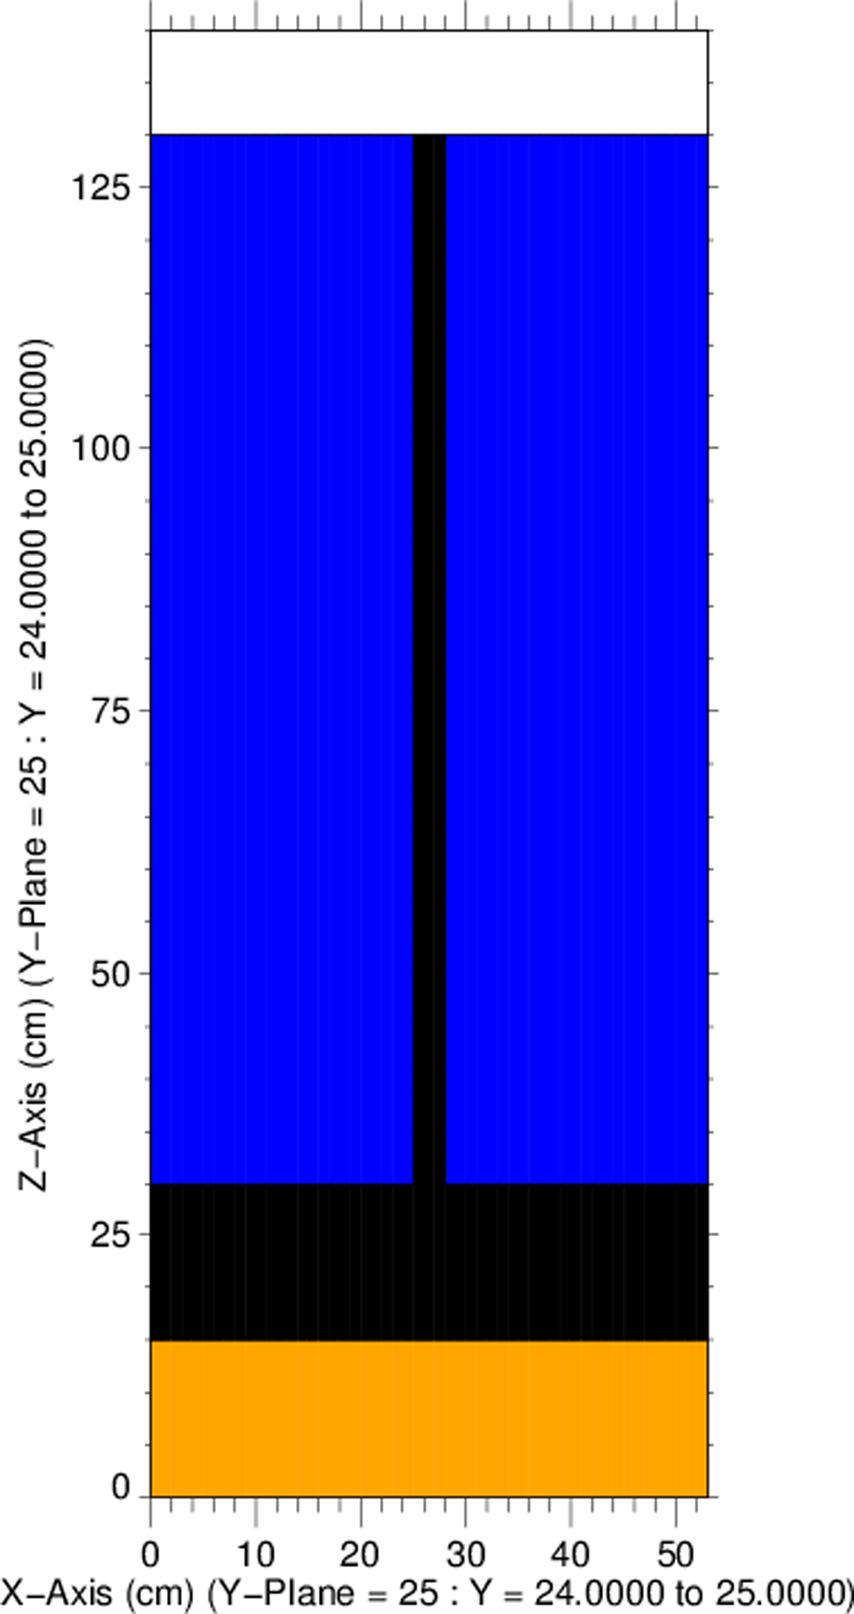
\includegraphics[width=0.4\textwidth]{img/steel-xz.png}
\caption{Steel plate in water geometry ($x-z$ slice through $y = 25$ cm) 
         \cite{wilsonslaybaugh}.}
\label{steelxz}
\end{figure}

The problem measurements are $53\times50\times140$ cm. The scenario is uniform 
in the $y$-direction and materials vary mainly in the $z$-direction. The source
region extends from 0 to 15 cm, the steel shield extends between 15 and 30 cm, 
the water and steel plate extend from 30 to 130 cm, and the air extends from 
130 to 140 cm. The steel plate is 3 cm wide and is centered at $x = 26.5$ cm. 
Vacuum boundary conditions were used at the problem boundaries.

A non-uniform Cartesian mesh was used for the spatial discretization in the 
deterministic calculations. In the $x$-direction, voxel width is 5 cm between
$x = 0$ cm and $x = 25$ cm, 0.5 cm between $x = 25$ cm and $x = 28$ cm, and 5 
cm between $x = 28$ cm and $x = 53$ cm. A uniform spacing of voxel width 1 cm 
was used in the $y$-direction. In the $z$-direction, the spatial cell width is
3 cm between $z = 0$ cm and $z = 30$ cm and 2 cm between $z = 30$ cm and 
$z = 140$ cm.

\begin{table}[!htb]
\centering
\caption{Materials and compositions in the steel plate in water scenario.}
\label{steel-mat}
\begin{tabular}{l|cc}
\textbf{Material} & \multicolumn{2}{c}{\textbf{Isotopes (Atomic \%)}} \\ \hline
\multirow{5}{*}{Source}   & U-235   & (0.000247) \\
                          & U-238   & (0.009287) \\
                          & Zr-nat. & (0.004009) \\
                          & H-1     & (0.037394) \\
                          & O-16    & (0.034927) \\ \hline
\multirow{4}{*}{Air}      & N-14    & (0.784431) \\
                          & O-16    & (0.210748) \\
                          & Ar-nat. & (0.004671) \\
                          & C-nat.  & (0.000150) \\ \hline
\multirow{2}{*}{Carbon Steel} & C-nat.  & (0.022831) \\
                              & Fe-nat. & (0.977169) \\ \hline
\multirow{2}{*}{Water}        & H-1     & (2)        \\
                              & O-16    & (1)        \\
\end{tabular}
\end{table}

The composition of the neutron source block is a homogenization of water,
zirconium, and uranium and was calculated based on the geometry and composition
of the Rowlands UO$_2$ pin cell benchmark specification \cite{pincell}. The
source is a U-235 fission 
spectrum that is uniformly distributed throughout the homogenized material. The
compositions of air, carbon steel, and water were taken from the Compendium of 
Material Composition Data for Radiation Transport Modeling \cite{pnnl}.

%%---------------------------------------------------------------------------%%
\subsection{Dog-Legged Void Neutron (DLVN)}

The next problem modeled is the dog-legged void neutron (DLVN) experimental 
benchmark, which was designed to measure neutron streaming in iron with air
voids. The model used in the following calculations was constructed from
References \cite{sw-dlvn,j-dlvn,dlvn1991}. The two materials used in the
problem are elemental iron and polyethylene. The polyethylene composition used
was C$_2$H$_4$. This is listed as ``polyethylene, non-borated'' and is material
248 in Reference \cite{pnnl}. 

\begin{figure}[!htb]
\centering
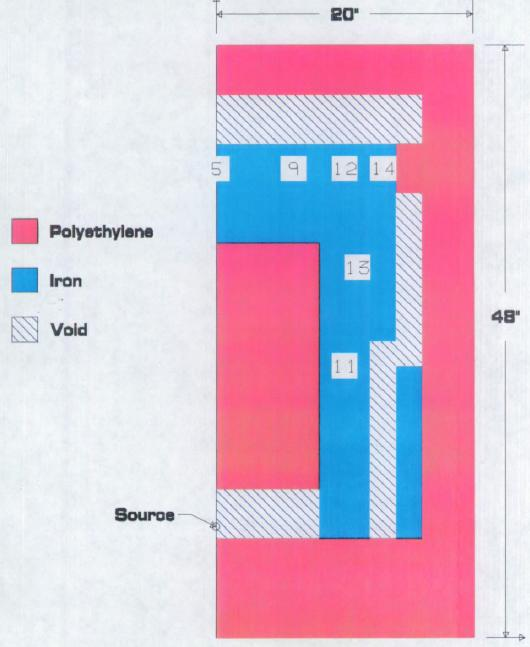
\includegraphics[width=0.5\textwidth]{img/dlvn.png}
\caption{Centerline cutaway of DLVN setup \cite{sw-dlvn}.}
\label{dlvn}
\end{figure}

The problem measurements are $40\times54\times48$ inches. A uniform spatial
mesh was imposed over the entire problem, with voxels measuring 1 inch per side.
The neutron source in this problem is a Cf-252 point source located at the 
center of the $x-$ and $y-$directions and at $z = 9$ inches.
This point source was approximated as a small volumetric source in the tests in
this work.

The experimental configuration is symmetric about the $y-z$ plane at $x = 0$
and so is usually simulated with a reflecting boundary at $x = 0$ and vacuum
boundaries on all other sides of the configuration. For the tests in this work,
the use of reflecting boundary conditions was not available, so the model used 
was constructed to represent the entire experimental geometry configuration.
Vacuum boundary conditions were applied to the outside of the entire problem.

%%---------------------------------------------------------------------------%%
\subsection{Simplified Portal Monitor}

The final problem described here is a simplified portal monitor scenario.
Portal monitors are large detector panels used to screen cargo for illicit
radioactive materials. The problem models a cargo container holding a Ba-133
photon point source and large blocks of homogenized iron and polyethylene. 
The geometry and material configuration used in this test is the same as the
example problem listed in Section 7.2 of the ADVANTG technical report
\cite{advantg}. Diagrams of the simplified portal monitor problem are shown in
Figure \ref{p1}.

\begin{figure}[!htb]
\centering
\begin{subfigure}{0.475\textwidth}
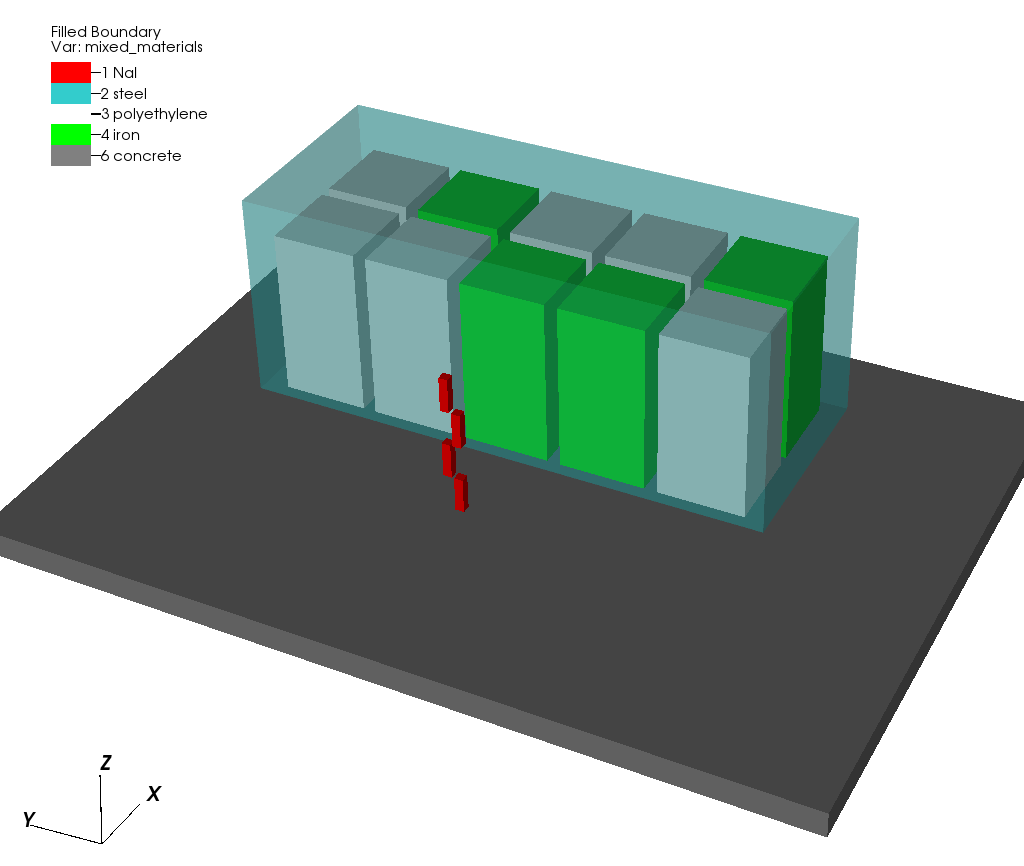
\includegraphics[width=\textwidth]{img/portal1.png}
\end{subfigure}
\begin{subfigure}{0.475\textwidth}
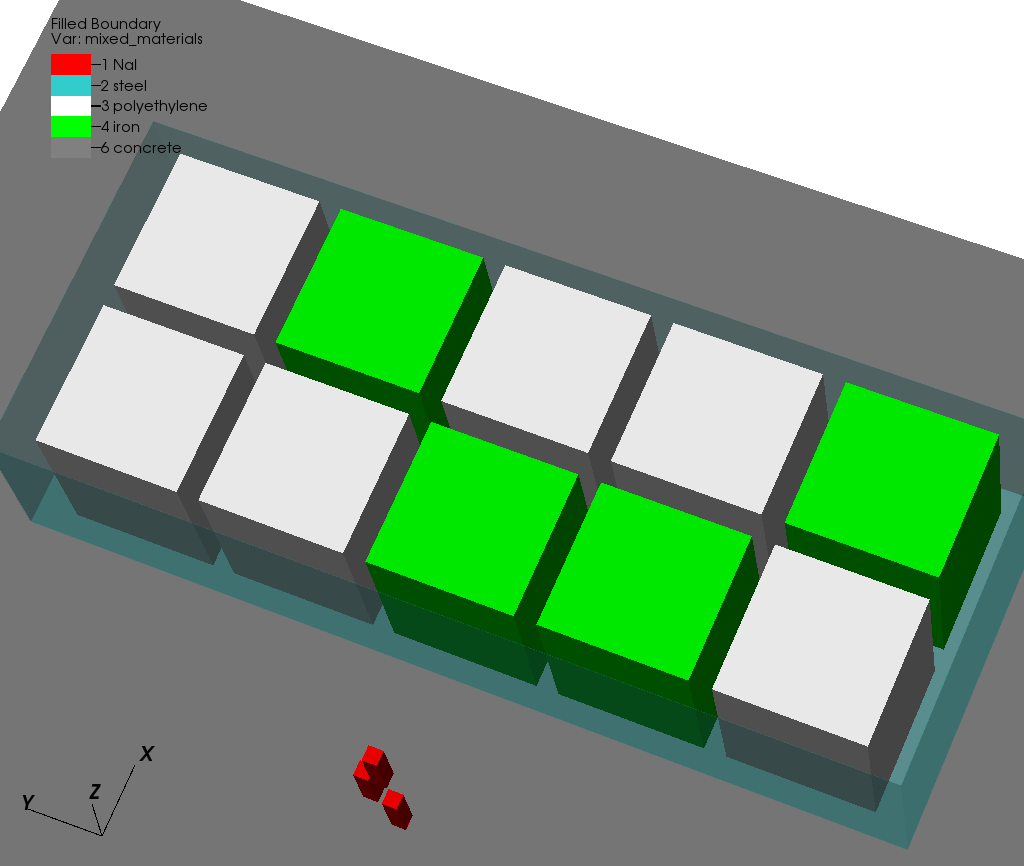
\includegraphics[width=\textwidth]{img/portal2.png}
\end{subfigure}
\caption{Top and side views of simplified portal problem \cite{advantg}.}
\label{p1}
\end{figure}

In Figure \ref{p1}, the different colors represent different materials. The NaI
detectors are red and the gray material is concrete. The two types of material
blocks are iron, shown in green, and polyethylene, shown in white. The steel
cargo container surrounds the particle source and material blocks and is a
semitransparent blue.

A non-uniform Cartesian mesh that captures all of the problem's material
boundaries was constructed for this simulation. The voxels are nominally 10 cm
thick within the cargo container. Additional mesh planes parallel to the
$x-$axis were added to the gaps between the homogenized iron and polyethylene
blocks \cite{advantg}. Vacuum boundary conditions are present at all problem
edges.

%%---------------------------------------------------------------------------%%
\subsection{Calculation Parameters}

All of the deterministic calculations used 32 processes on a 2.8GHz AMD 
Opteron\texttrademark\ 6320 Processor \cite{amd}, two for each logical CPU
unit. With this in mind, all deterministic calculations were set to use the
same Denovo computational block structure of 8 blocks 
in the $x-$dimension, 4 blocks in the $y-$dimension, and 1 block in the 
$z-$dimension; thus the total number of computational blocks equals the number
of processes. Denovo uses the Koch-Baker-Alcouffe (KBA) parallel sweep
algorithm for high parallel efficiency in calculating transport sweeps
\cite{denovo}; the aforementioned block structure was chosen to achieve the
same parallel decomposition among all test case deterministic simulations. 

The two neutron transport test cases use the same coarse energy group structure
specified in  the ``27n19g'' library; the groups in this library are listed in 
Table A-1 of Appendix A of the ADVANTG technical report \cite{advantg}.
The simplified portal monitor scenario uses a truncated version of the library;
the highest energy emission line of Ba-133 is 383.8 keV, so the highest energy
group of the calculations was set to group number 41, which has an upper energy
of 400 keV \cite{advantg}. Because 
energy discretization is treated the same way between the traditional discrete
ordinates formulation and the LDO equations, it was assumed that energy group 
structure would not greatly impact the comparative results.
The step characteristics (SC) spatial discretization was used in all of the
calculations and all cases used a P$_5$ scattering expansion.

We compare the LDO equations' solutions with those from quadruple range (QR),
Galerkin, and linear-discontinuous finite element (LDFE) quadrature sets.
For the comparisons presented here, quadrature sets of similar angular mesh
refinement were chosen such that the quadrature sets have approximately the 
same total number of angles, with the exception of the Galerkin quadrature set.
The QR quadrature set is of order 4 and has 128 angles, the LDFE set is order 1
with 128 angles, and the LDO set is of order 11 with 144 angles. 
The Galerkin quadrature set chosen as the representative example here is of
order 4 and has 24 angles. This set was chosen because its corresponding \pn\
order is 5 and so the scattering data used matches that of the other quadrature
types. At the time of this writing, Galerkin quadrature sets are implemented in
the Exnihilo framework with the restriction that the \pn\ order be one greater
than the \sn\ order.

%---------------------------------------------------------------------------%%
\section{Results}
\label{sec:results}

We present descriptions of and numerical results corresponding to three test
case scenarios. The first two scenarios are neutron transport problems, while
the third scenario is a photon transport problem. Flux calculations from the
four quadrature types are presented for each test case, with comparisons
highlighted between the LDO flux solutions and those of the standard
quadrature types.

%---------------------------------------------------------------------------%%
\subsection{Steel Plate Embedded in Water}

Figure \ref{steel-fwd-slices} shows a scalar flux slice plot for each
quadrature type for the steel plate scenario.  Each of the flux slices is at
the midplane of the $y-$dimension such that $y = 25$ cm. The geometry/material
borders are outlined on each plot as well. All plots show the same expected
result -- the scalar flux is highest in the source region and drops off by
orders of magnitude along the $z-$axis.

To more thoroughly evaluate the LDO quadrature set in this test case, we will
look more closely at the differences between the LDO flux and
the three other quadrature types. Figure \ref{steel-fwd-diff-rel} shows three
plots of relative flux differences; each plot compares the LDO
flux to the flux from one of the standard quadrature set types. The relative
flux difference is calculated as

\begin{equation}
\phi_{\mathrm{diff}} = 
\frac{\left|\phi_{\mathrm{LDO}}-\phi_{\mathrm{ref}}\right|}{\phi_{\mathrm{ref}}}\:,
\label{flux-diff}
\end{equation}

\noindent where $\phi_{\mathrm{ref}}$ is the scalar flux calculated using the 
standard quadrature set and is taken to be the reference value. For all three
of the standard quadrature sets, the area of greatest agreement with the LDO
scalar flux is towards the bottom of the problem geometry, with discrepancies
growing along the $z-$axis. The greatest difference can be seen between the LDO
and Galerkin quadrature sets, while the LDO and QR quadrature sets agree best.
The area of greatest discrepancy between the QR and LDO flux solutions is in
the region of air just beyond the steel beam. We note here that this particular
deviation is most likely due to issues in processing iron cross section data
inherent to deterministic calculations \cite{wilsonslaybaugh}.

Table \ref{steel-fwd-diff-table} lists the minimum, maximum, and average
differences between various quadrature types for the flux slices plotted in
Figure \ref{steel-fwd-diff-rel}. We compare the representative LDO flux
solution to the solutions from the three standard representative quadrature
types and also compare the Galerkin and LDFE results against the QR result. On
average, the LDO scalar flux solution matches the QR flux solution more
closely than it matches either the Galerkin or LDFE flux solutions.
Additionally, the LDO flux solution matches the QR flux solution more closely
than do either of the Galerkin and LDFE flux solutions.

\begin{table}[!hbt]
\centering
\caption{Steel plate scalar flux extremal and average relative differences.}
\label{steel-fwd-diff-table}
\begin{tabular}{l|ccc}
\textbf{Comparison} & \textbf{Min. Diff.} & \textbf{Max. Diff.} & \textbf{Avg. Diff.} 
\\ \hline
LDO/QR              & 6\E{-6}             & 1.0913\E{-1}       & 2.206\E{-2}
\rule{0pt}{2.6ex} \\ 
LDO/Galerkin        & 2\E{-5}             & 4.5132\E{0}        & 9.303\E{-1}      \\
LDO/LDFE            & 5\E{-7}             & 2.7850\E{-1}       & 9.418\E{-2}      \\
Galerkin/QR         & 3\E{-5}             & 8.2364\E{-1}       & 2.903\E{-1}      \\
LDFE/QR             & 2\E{-7}             & 2.4807\E{-1}       & 9.632\E{-2}
\end{tabular}
\end{table}

Looking at Figures \ref{steel-fwd-slices} and \ref{steel-fwd-diff-rel}, we
note that the  scalar flux solutions from the LDO equations capture the same
physical trends as the standard quadrature type solutions and also that the
LDO flux solution most closely matches that using the QR quadrature set.
Additionally, Table \ref{steel-fwd-diff-table} shows an average difference of
2.2\% between the plotted flux solutions from the representative LDO and QR
quadrature sets, which is the lowest average difference seen in the
comparisons here. As QR quadratures are commonly used in \sn\ calculations,
the relative agreement of the LDO scalar flux with the QR scalar flux
motivates further exploration of the LDO scalar flux solutions.

\begin{figure}[!htb]
\centering
\begin{subfigure}{0.4\textwidth}
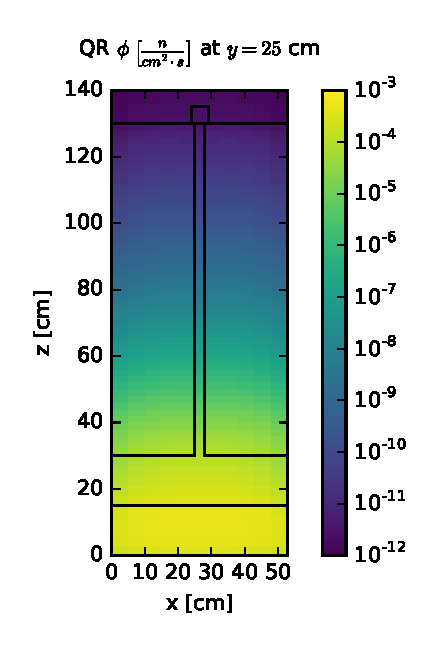
\includegraphics[max height=0.445\textheight]
{img/steel-fwd-flux-qr04.eps}
\subcaption{QR scalar flux slice.}
\end{subfigure} ~
\begin{subfigure}{0.4\textwidth}
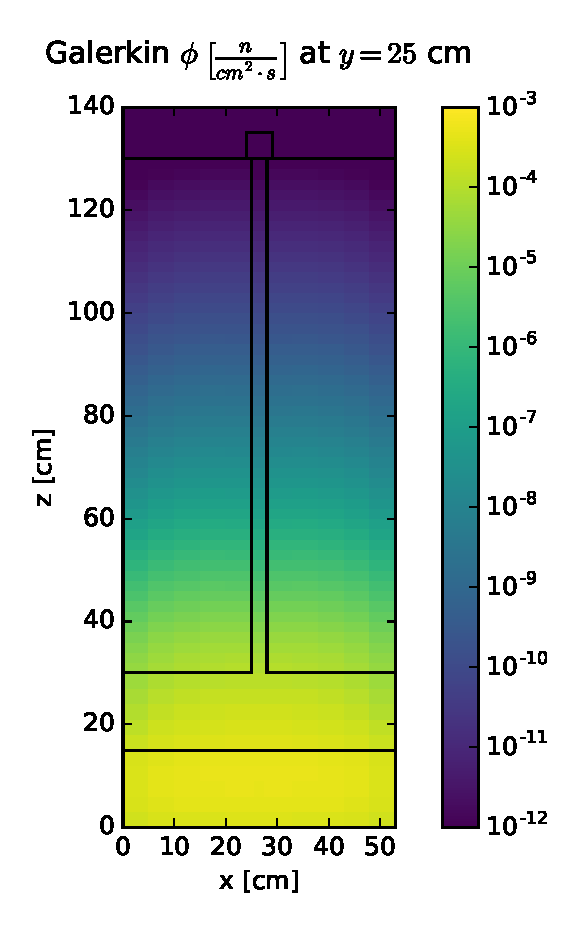
\includegraphics[max height=0.445\textheight]
{img/steel-fwd-flux-gkn04.eps}
\subcaption{Galerkin scalar flux slice.}
\end{subfigure}
\\
\begin{subfigure}{0.4\textwidth}
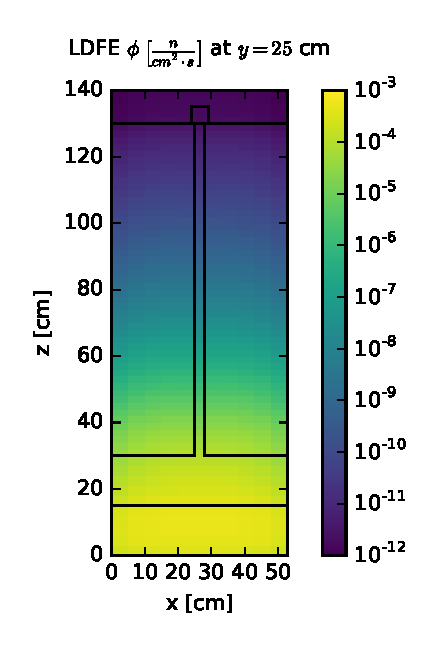
\includegraphics[max height=0.445\textheight]
{img/steel-fwd-flux-ldfe01.eps}
\subcaption{LDFE scalar flux slice.}
\end{subfigure} ~
\begin{subfigure}{0.4\textwidth}
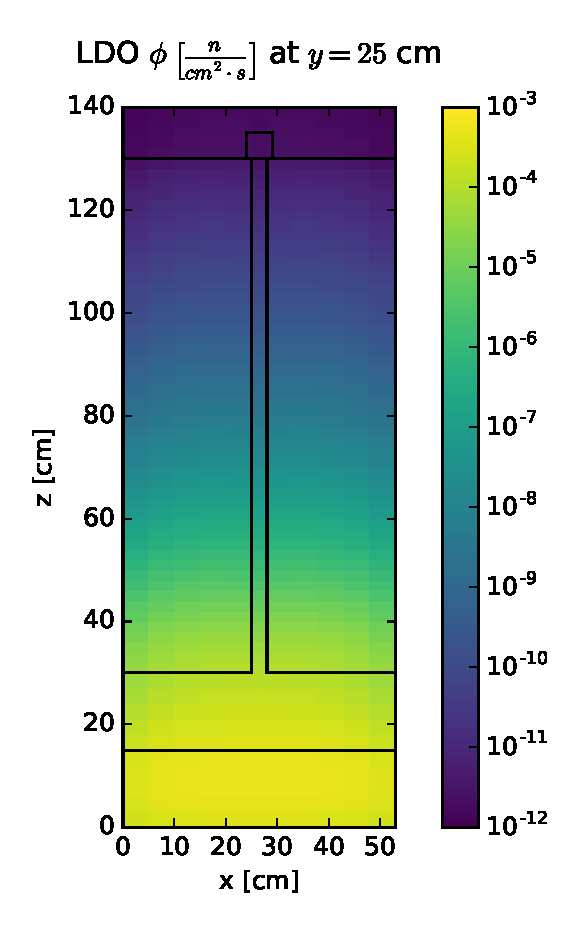
\includegraphics[max height=0.445\textheight]
{img/steel-fwd-flux-ldo11.eps}
\subcaption{LDO scalar flux slice.}
\end{subfigure}
\caption{Steel plate scalar flux slices.}
\label{steel-fwd-slices}
\end{figure}

\begin{figure}[!htb]
\centering
\begin{subfigure}{0.4\textwidth}
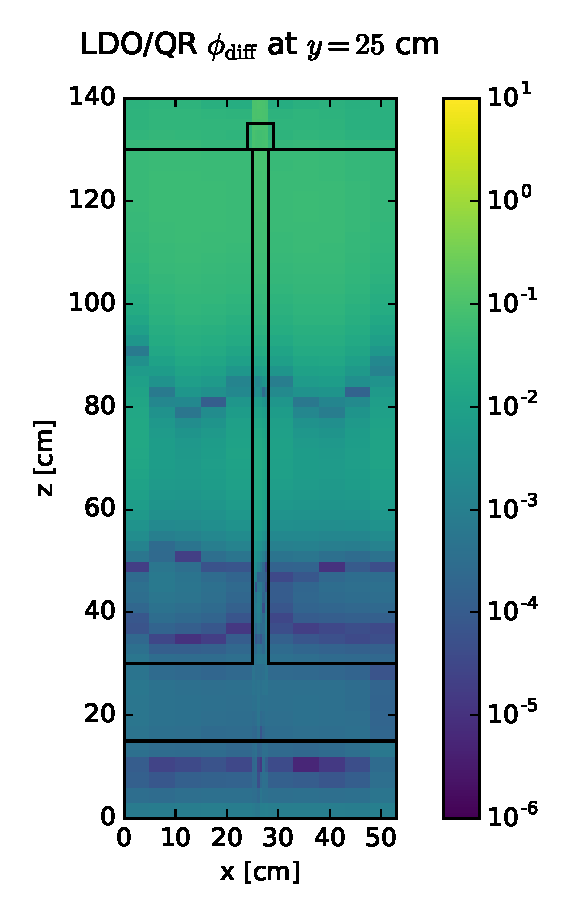
\includegraphics[max height=0.445\textheight]
{img/steel-flux-diff-qr.eps}
\subcaption{LDO/QR flux rel. diff.}
\end{subfigure} ~
\begin{subfigure}{0.4\textwidth}
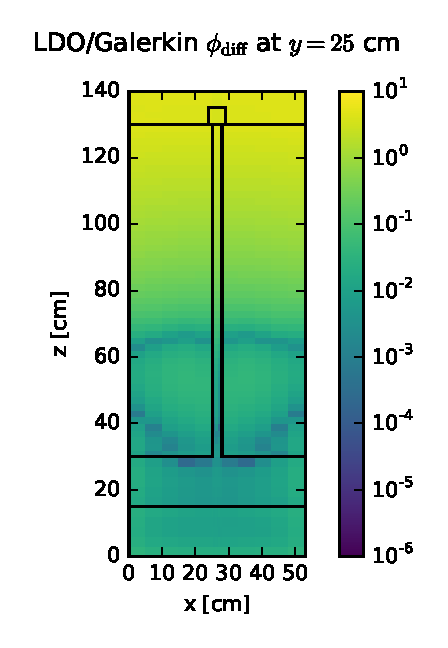
\includegraphics[max height=0.445\textheight]
{img/steel-flux-diff-gkn.eps}
\subcaption{LDO/Galerkin flux rel. diff.}
\end{subfigure}
\\
\begin{subfigure}{0.4\textwidth}
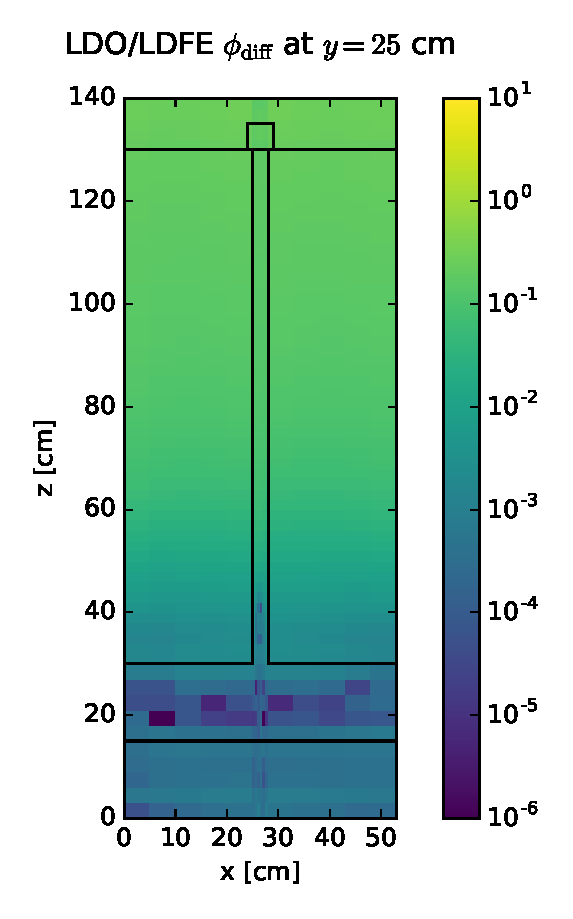
\includegraphics[max height=0.445\textheight]
{img/steel-flux-diff-ldfe.eps}
\subcaption{LDO/LDFE flux rel. diff.}
\end{subfigure}
\caption{Steel plate  scalar flux relative difference slices.}
\label{steel-fwd-diff-rel}
\end{figure}

\FloatBarrier
%---------------------------------------------------------------------------%%
\subsection{Dog-Legged Void Neutron (DLVN)}

For the DLVN test case, we present flux slice plots for the same representative
quadrature sets. Although the entire DLVN
experimental geometry was simulated, here we plot only half of the
configuration; this is the typical view of the benchmark seen in the
literature.

Figure \ref{dlvn-fwd-slices} shows the scalar flux for each of the
representative quadrature sets at the midplane of $y = 27$ inches (68.58 cm).
Each of the plots has outlines of the material boundaries with the detector
locations delineated as well. As expected, the flux is highest at the neutron
source and decreases as particles move through the experimental configuration.
With this, we again look at the differences between the representative LDO flux
and the three other quadrature types. 

As with the previous test case, the flux differences 
are calculated with Equation \ref{flux-diff}. In the DLVN scenario, the 
differences stem from the source location. This is not surprising; the particle
source here is approximately a point source and so these differences appear in
the form of ray effects, where the discrete angles in the LDO quadrature set do
not overlap with the angles in a given standard quadrature set. Similar to the
steel plate in water test case, the LDO scalar flux best matches the QR scalar
flux and the largest differences are seen between the LDO and Galerkin scalar
flux plots. Looking at Figure \ref{dlvn-fwd-diff-gkn}, the areas of greatest
discrepancy appear as ray effects; the relative coarseness of the
representative Galerkin quadrature set angular mesh is likely the cause of
this. This is visibly pronounced in the DLVN case because of the geometrically
small particle source. Ray effects are also likely the source of the 
LDO/Galerkin discrepancy seen for the steel plate embedded in water, but
they are lessened in that scenario by the larger volumetric source.

Lastly, it is instructive to compare the results of the deterministic
scalar flux solutions with the experimentally measured flux values at the
detector locations. Table \ref{dlvn-fwd-det} lists the experimentally measured
\cite{dlvn1991} and deterministically calculated scalar flux values at the
detector locations noted in Figure \ref{dlvn}. Table \ref{dlvn-fwd-det-diff}
lists the percent differences between the deterministically calculated flux
values and experimentally determined flux values with the lowest difference
for each detector location emphasized.

\begin{table}[!htb]
\centering
\caption{DLVN benchmark experimental and simulated scalar flux values [n/cm$^2$/s].}
\label{dlvn-fwd-det}
\begin{tabular}{l|ccccccc}
              & Det. \#5       & Det. \#9       & Det. \#11      & Det. \#12
              & Det. \#13      & Det. \#14 \\ \hline
Exp. Flux     & 6.97\E{-8}     & 1.57\E{-7}     & 8.81\E{-6}     & 2.60\E{-7}
              & 1.42\E{-6}     & 2.74\E{-7}     \rule{0pt}{2.6ex} \\
QR            & 4.98\E{-8}     & 1.68\E{-7}     & 8.65\E{-5}     & 4.92\E{-7}
              & 2.71\E{-6}     & 1.45\E{-6}     \\
Galerkin      & 3.24\E{-8}     & 1.47\E{-7}     & 8.19\E{-5}     & 4.43\E{-7}
              & 2.95\E{-6}     & 9.55\E{-7}     \\
LDFE          & 5.12\E{-8}     & 1.76\E{-7}     & 9.17\E{-5}     & 5.14\E{-7}
              & 2.93\E{-6}     & 1.47\E{-6}     \\
LDO           & 4.56\E{-8}     & 1.39\E{-7}     & 7.88\E{-5}     & 4.28\E{-7}
              & 2.37\E{-6}     & 1.28\E{-6}
\end{tabular}
\end{table}

\begin{table}[!htb]
\centering
\caption{Percent differences between DLVN experimental and simulated scalar
         flux values.}
\label{dlvn-fwd-det-diff}
\begin{tabular}{l|ccccccc}
              & Det. \#5       & Det. \#9        & Det. \#11       & Det. \#12
              & Det. \#13      & Det. \#14       \\ \hline
QR            & \textbf{25.58} & 6.89            & 881.94          & 89.09
              & 90.63          & 428.81          \\
Galerkin      & 53.48          & \textbf{6.37}   & 829.72          & 70.56
              & 107.7         & \textbf{248.42} \\
LDFE          & 26.61          & 12.3           & 940.41          & 97.75
              & 106.4         & 435.01          \\
LDO           & 34.61          & 11.2           & \textbf{794.75} & \textbf{64.46}
              & \textbf{66.77} & 368.24
\end{tabular}
\end{table}

Looking at Table \ref{dlvn-fwd-det-diff}, we see that all of the calculated
values fall outside of the experimental uncertainty of five percent
\cite{dlvn1991}. The results from the LDO quadrature set most closely match
the experimental results for half of the detector locations, which is better
than any of the standard quadrature types tested here. Table \ref{dlvn-fwd-
diff-table} lists the extreme and average values of the scalar flux relative
difference slices shown in Figure \ref{dlvn-fwd-diff-rel}, with Galerkin/QR
and LDFE/QR comparisons included for reference. We see that, on average, the
LDO flux solution matches the QR flux solution better than it matches those of
the other quadrature types. However, in this case, the LDFE flux solution
matches the QR flux solution on average better than any other quadrature type,
including the LDO flux solution (5\% difference versus 8.4\% difference).

\begin{table}[!hbt]
\centering
\caption{DLVN benchmark scalar flux extremal and average relative 
         differences.}
\label{dlvn-fwd-diff-table}
\begin{tabular}{l|ccc}
\textbf{Comparison} & \textbf{Min. Diff.} & \textbf{Max. Diff.} & \textbf{Avg. Diff.} 
\\ \hline
LDO/QR              & 2\E{-4}             & 8.3986\E{-1}  & 8.436\E{-2} \rule{0pt}{2.6ex} \\ 
LDO/Galerkin        & 1\E{-6}             & 2.1395\E{0}   & 2.419\E{-1}      \\
LDO/LDFE            & 3\E{-5}             & 8.7127\E{-1}  & 1.166\E{-1}      \\
Galerkin/QR         & 3\E{-4}             & 6.3722\E{-1}  & 1.924\E{-1}      \\
LDFE/QR             & 3\E{-5}             & 2.6688\E{-1}  & 5.047\E{-2}
\end{tabular}
\end{table}

\begin{figure}[!htb]
\centering
\begin{subfigure}{0.4\textwidth}
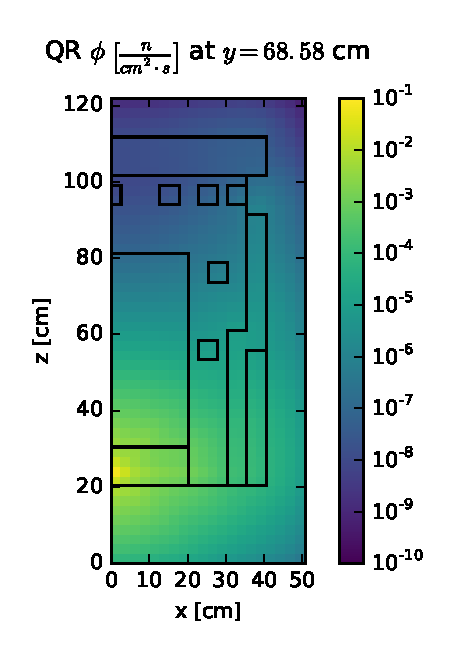
\includegraphics[max height=0.445\textheight]
{img/dlvn-fwd-flux-qr04.eps}
\subcaption{QR scalar flux slice.}
\end{subfigure} ~
\begin{subfigure}{0.4\textwidth}
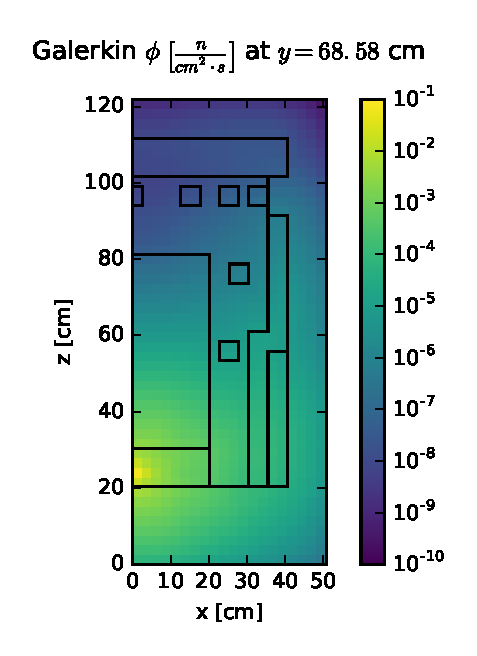
\includegraphics[max height=0.445\textheight]
{img/dlvn-fwd-flux-gkn04.eps}
\subcaption{Galerkin scalar flux slice.}
\end{subfigure}
\\
\begin{subfigure}{0.4\textwidth}
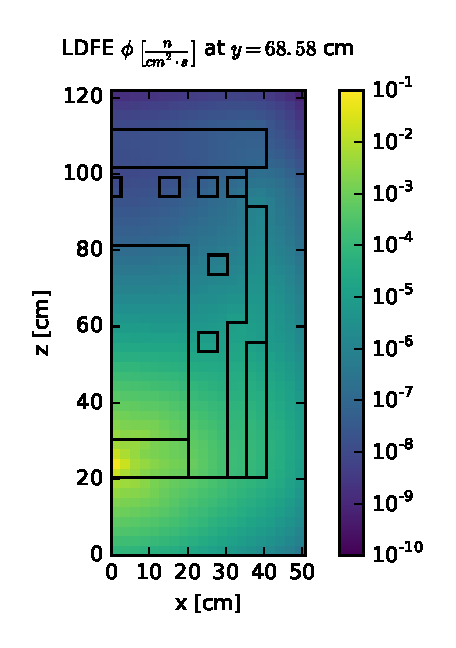
\includegraphics[max height=0.445\textheight]
{img/dlvn-fwd-flux-ldfe01.eps}
\subcaption{LDFE scalar flux slice.}
\end{subfigure} ~
\begin{subfigure}{0.4\textwidth}
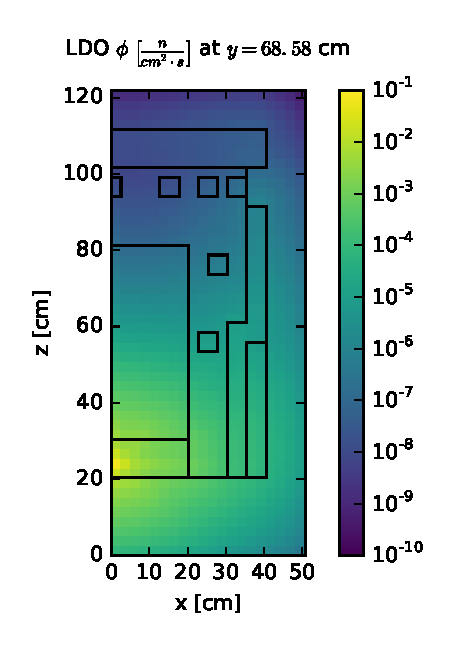
\includegraphics[max height=0.445\textheight]
{img/dlvn-fwd-flux-ldo11.eps}
\subcaption{LDO scalar flux slice.}
\end{subfigure}
\caption{DLVN benchmark scalar flux slices.}
\label{dlvn-fwd-slices}
\end{figure}

\begin{figure}[!hbt]
\centering
\begin{subfigure}{0.4\textwidth}
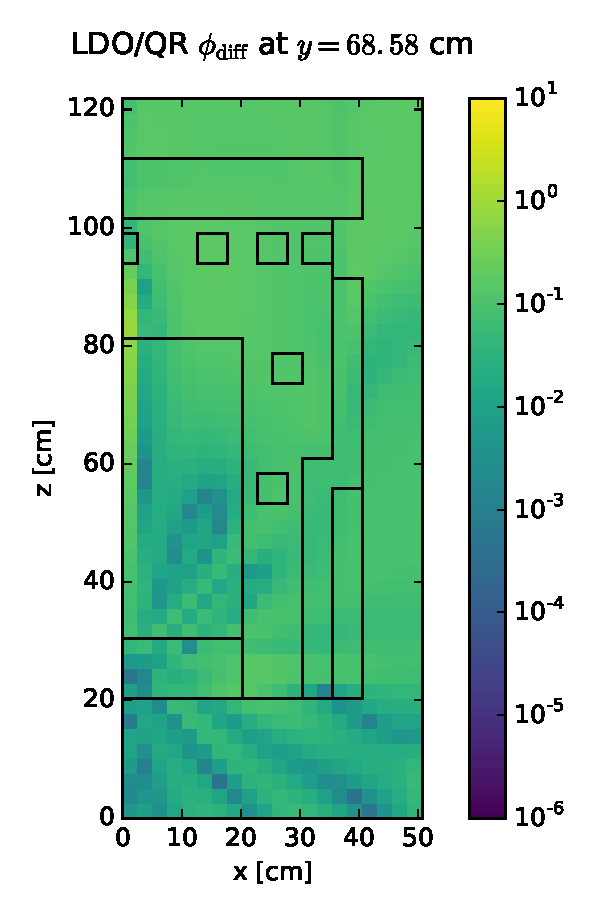
\includegraphics[max height=0.445\textheight]
{img/dlvn-flux-diff-qr.eps}
\subcaption{LDO/QR flux rel. diff.}
\end{subfigure} ~
\begin{subfigure}{0.4\textwidth}
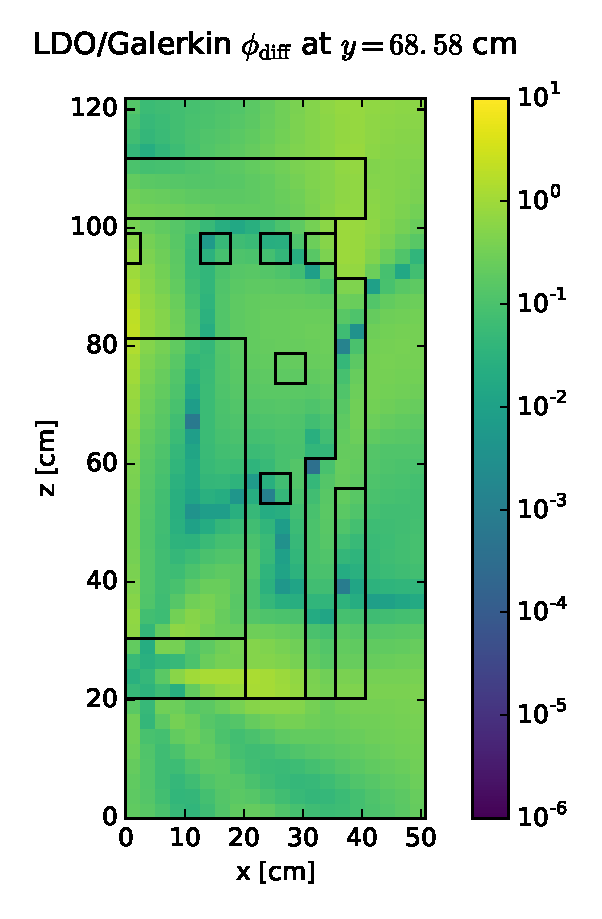
\includegraphics[max height=0.445\textheight]
{img/dlvn-flux-diff-gkn.eps}
\subcaption{LDO/Galerkin flux rel. diff.}
\label{dlvn-fwd-diff-gkn}
\end{subfigure}
\\
\begin{subfigure}{0.4\textwidth}
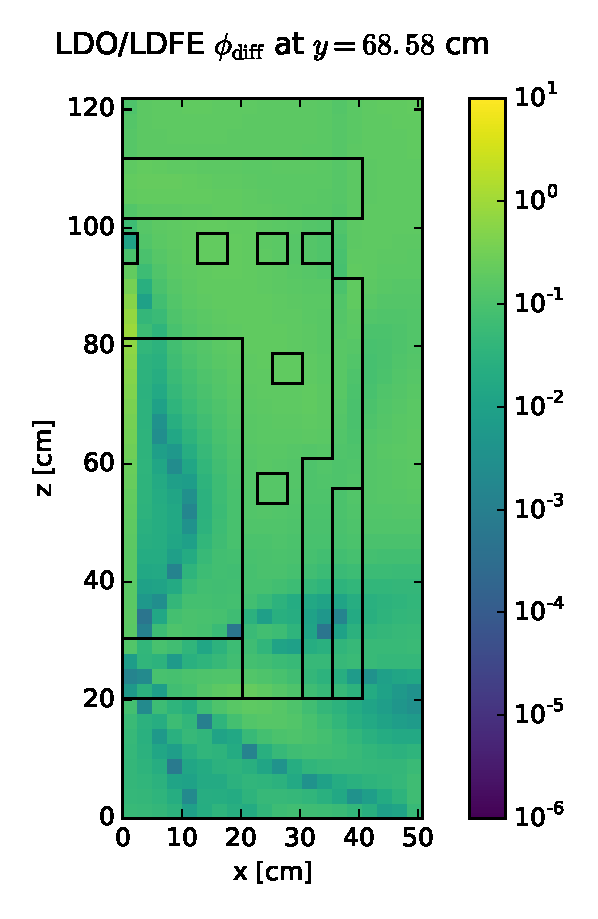
\includegraphics[max height=0.445\textheight]
{img/dlvn-flux-diff-ldfe.eps}
\subcaption{LDO/LDFE flux rel. diff.}
\end{subfigure}
\caption{DLVN benchmark scalar flux relative difference slices.}
\label{dlvn-fwd-diff-rel}
\end{figure}

\FloatBarrier
%%---------------------------------------------------------------------------%%
\subsection{Simplified Portal Monitor}

Lastly, we look at the simplified portal monitor problem with the small photon
source. Of the test cases presented here, the flux solutions differ most
greatly for this problem. Figure \ref{cargo-fwd-slices} shows scalar flux
solutions for the representative quadrature sets with the material pallets,
detector array, and shipping container outlines overlaid on the plots. Flux
slices are plotted at the midplane of $z = 243.84$ cm (96 inches). All of the
flux solutions plotted in Figure \ref{cargo-fwd-slices} display ray effects
as a result of the streaming paths created by the material variation of the
pallets inside of the shipping container.

As with the previous test cases, we look at the differences between the 
LDO flux and the three other quadrature types. In Figure
\ref{cargo-fwd-diff-rel}, the differences largely appear as ray effects. This
is unsurprising given the combination of the small volume of the photon 
source in the problem and the inherent difficulty of accurately simulating
particle streaming in deterministic calculations. Again, we see that the LDO
scalar flux solution exhibits strong disagreement with the Galerkin scalar
flux solution. The LDO/QR and LDO/LDFE comparison plots show discrepancies of
similar orders of magnitude, and all of the relative difference plots exhibit
the greatest difference along the $y-z$ plane streaming pathway located in the
center of the shipping container.

Table \ref{cargo-fwd-diff-table} lists the minimum, maximum, and average
values of the relative differences in the scalar flux solutions, shown in
Figure \ref{cargo-fwd-diff-rel}. As with all of the previous cases,
comparisons between the QR flux solution and the Galerkin and LDFE flux
solutions are included for reference. None of the flux solutions in this case
show particularly good agreement on average; the closest solutions are the
LDFE and QR flux solutions which have an average difference of about 24\%. Of
the three standard quadrature types, the LDO flux solution matches the QR flux
solution most closely. Given the localized small volumetric particle source
used in the problem in  combination with the streaming pathways created by the
scenario's material and geometry configuration, it is unsurprising that the
scalar flux solutions generated with the various quadrature sets show only
fair agreement.

\begin{table}[!hbt]
\centering
\caption{Portal monitor scalar photon flux extremal and average relative 
         differences.}
\label{cargo-fwd-diff-table}
\begin{tabular}{l|ccc}
\textbf{Comparison} & \textbf{Min. Diff.} & \textbf{Max. Diff.} & \textbf{Avg. Diff.} 
\\ \hline
LDO/QR              & 1\E{-6}             & 1.43357\E{2}           & 3.0683\E{-1}
\rule{0pt}{2.6ex}   \\
LDO/Galerkin        & 7\E{-5}             & 1.22385\E{2}           & 1.9609\E{0}      \\
LDO/LDFE            & 6\E{-5}             & 1.52743\E{2}           & 3.3349\E{-1}      \\
Galerkin/QR         & 4\E{-5}             & 2.46611\E{0}           & 3.9335\E{-1}      \\
LDFE/QR             & 2\E{-5}             & 2.09118\E{0}           & 2.3756\E{-1}
\end{tabular}
\end{table}

\clearpage
\begin{figure}[!htb]
\begin{subfigure}{\textwidth}
\centering
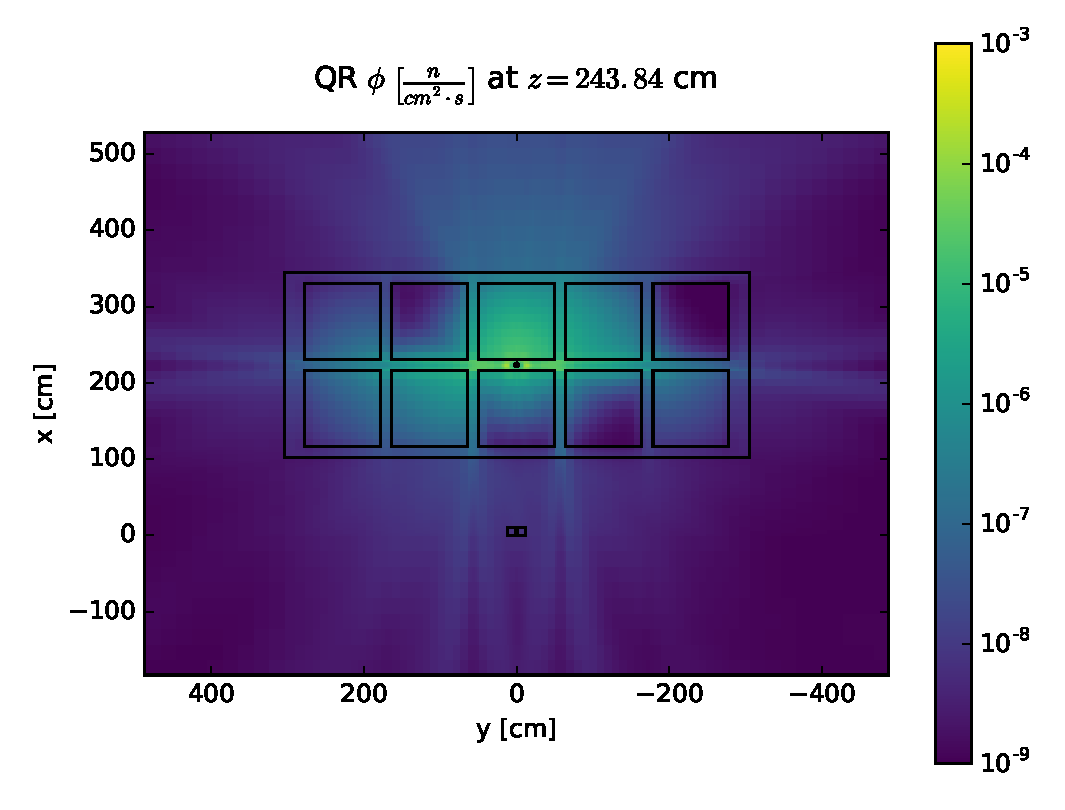
\includegraphics[max height=0.445\textheight]
{img/portal-fwd-flux-qr04.eps}
\subcaption{QR scalar flux slice.}
\end{subfigure}
\\
\begin{subfigure}{\textwidth}
\centering
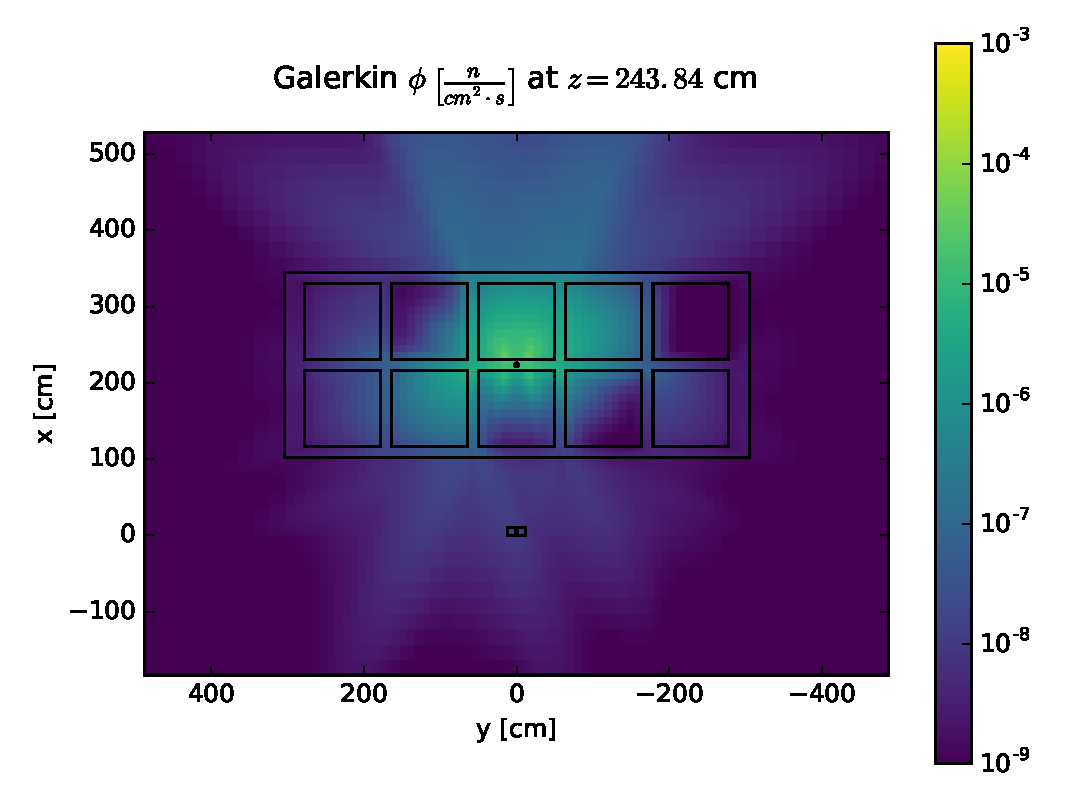
\includegraphics[max height=0.445\textheight]
{img/portal-fwd-flux-gkn04.eps}
\subcaption{Galerkin scalar flux slice.}
\end{subfigure}
\end{figure}
\clearpage
\begin{figure}[!htb]
\ContinuedFloat
\begin{subfigure}{\textwidth}
\centering
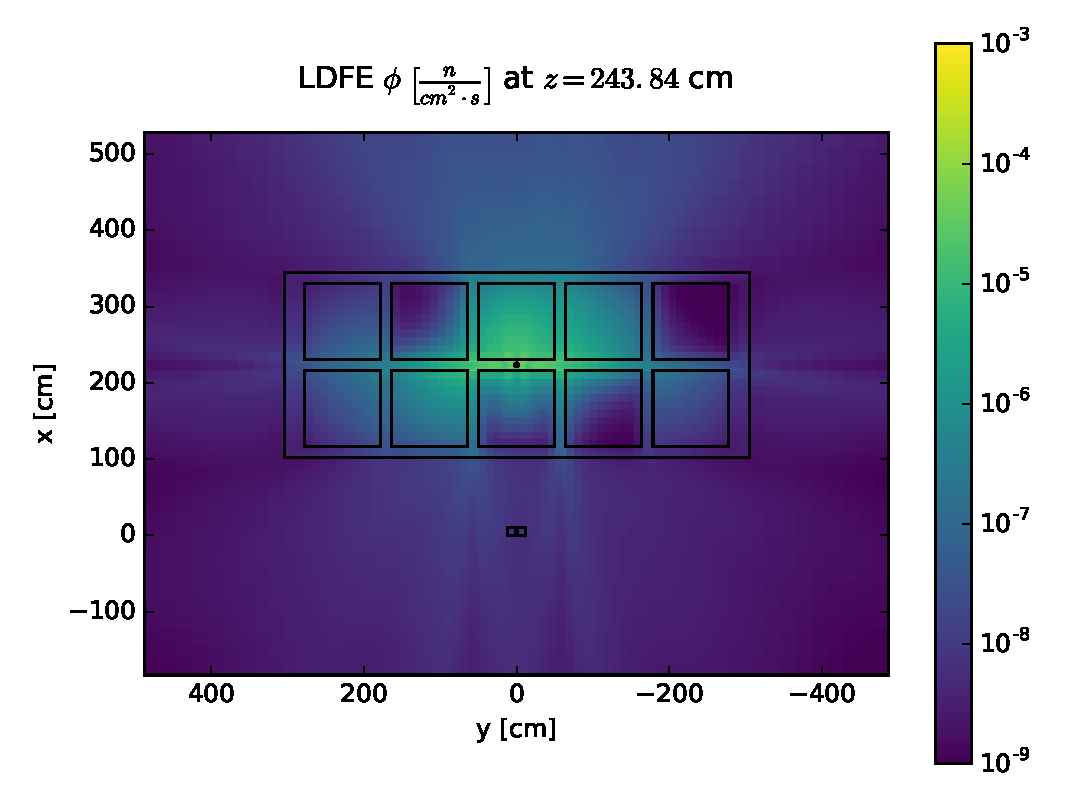
\includegraphics[max height=0.445\textheight]
{img/portal-fwd-flux-ldfe01.eps}
\subcaption{LDFE scalar flux slice.}
\end{subfigure}
\\
\begin{subfigure}{\textwidth}
\centering
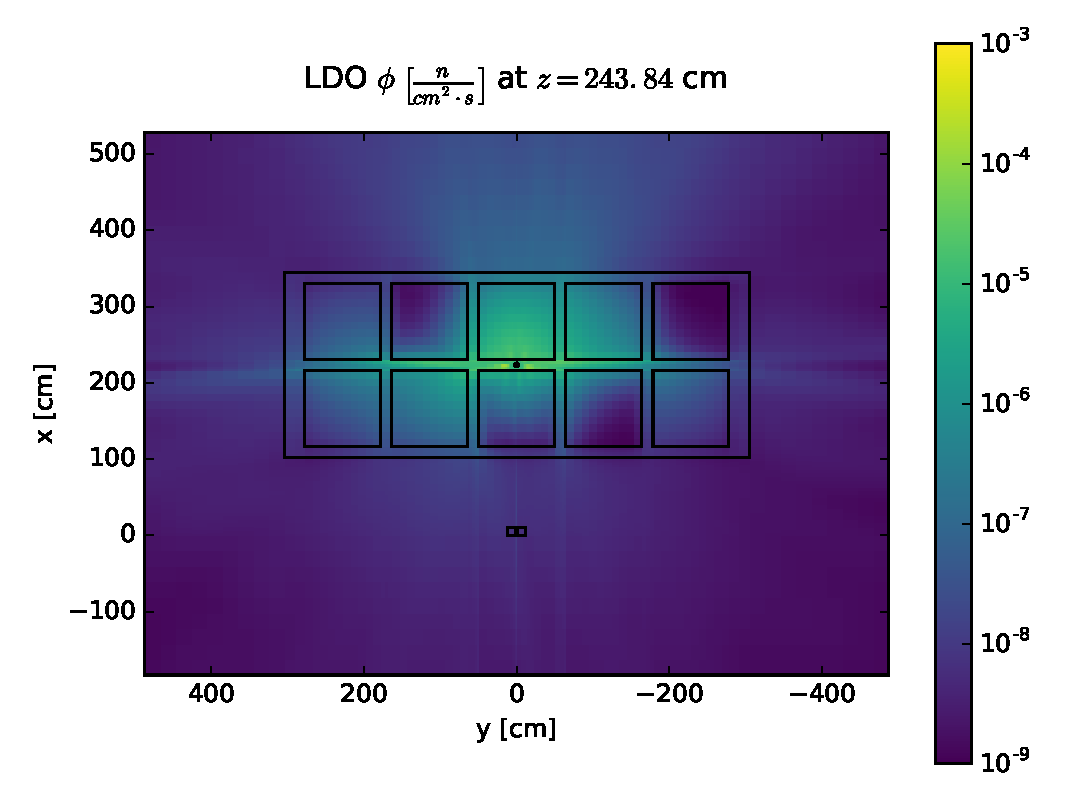
\includegraphics[max height=0.445\textheight]
{img/portal-fwd-flux-ldo11.eps}
\subcaption{LDO scalar flux slice.}
\end{subfigure}
\caption{Simplified portal monitor scenario scalar photon flux slices.}
\label{cargo-fwd-slices}
\end{figure}

\clearpage
\begin{figure}[!htb]
\begin{subfigure}{\textwidth}
\centering
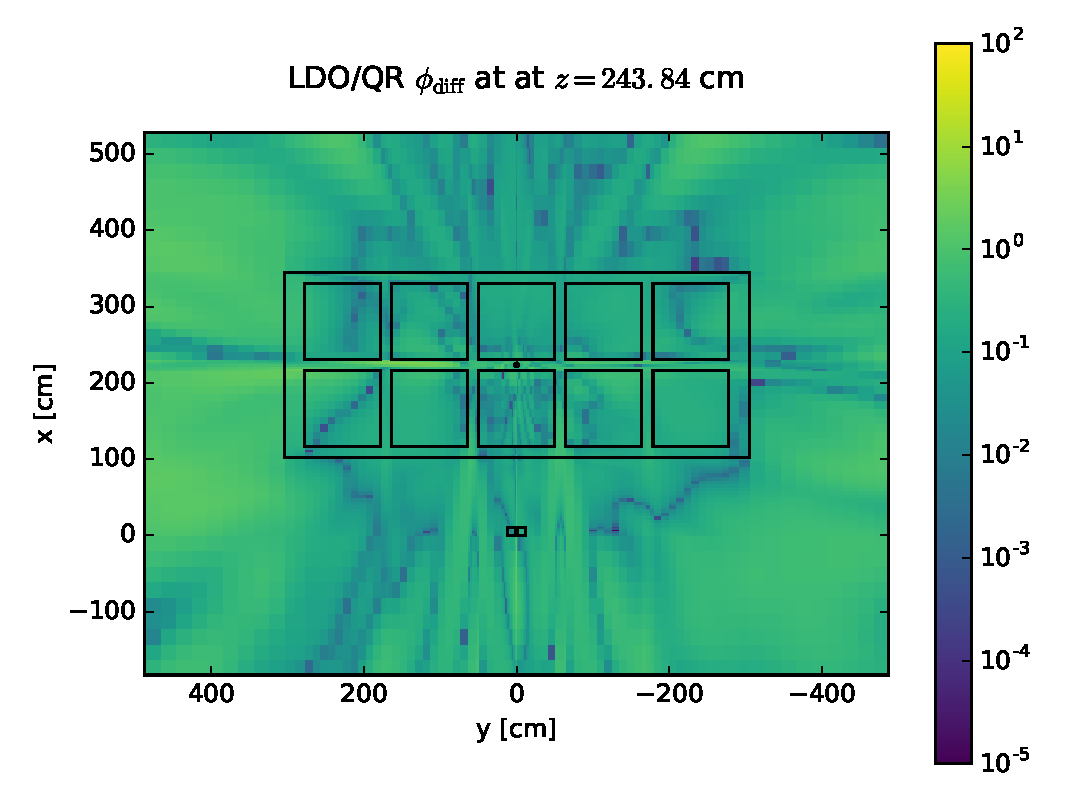
\includegraphics[max height=0.445\textheight]
{img/portal-flux-diff-qr.eps}
\subcaption{LDO/QR flux relative difference.}
\end{subfigure}
\\
\begin{subfigure}{\textwidth}
\centering
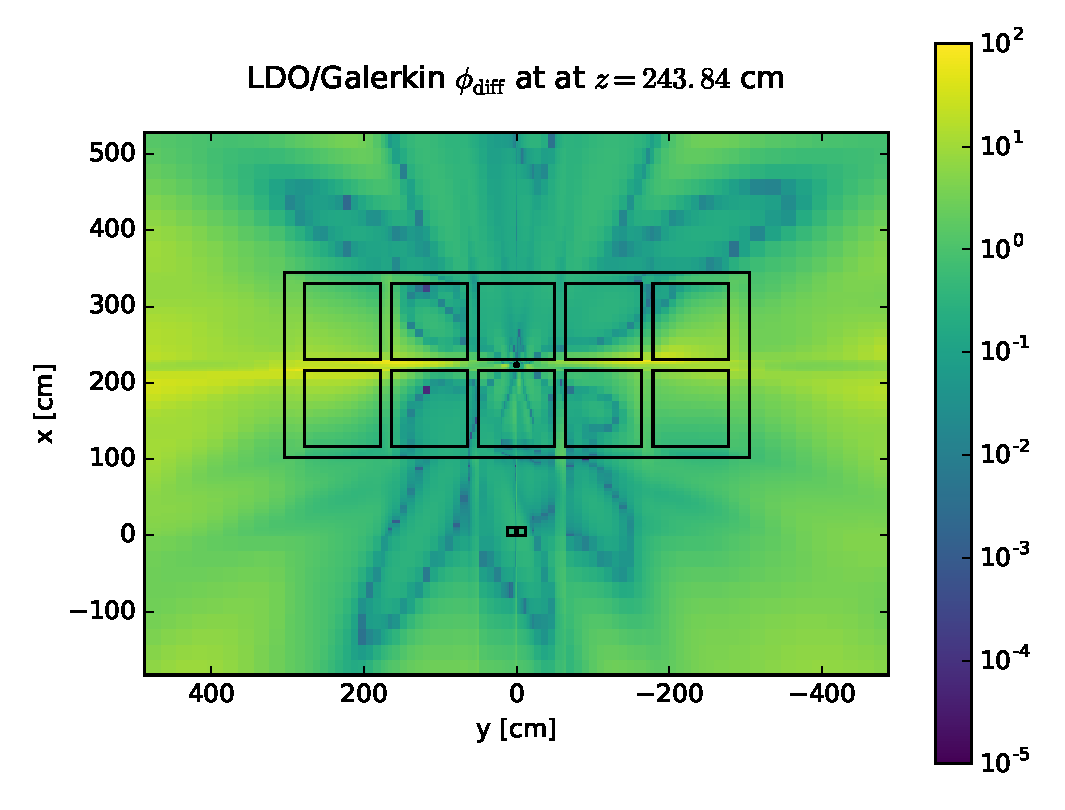
\includegraphics[max height=0.445\textheight]
{img/portal-flux-diff-gkn.eps}
\subcaption{LDO/Galerkin flux relative difference.}
\end{subfigure}
\end{figure}
\clearpage
\begin{figure}[!htb]
\ContinuedFloat
\begin{subfigure}{\textwidth}
\centering
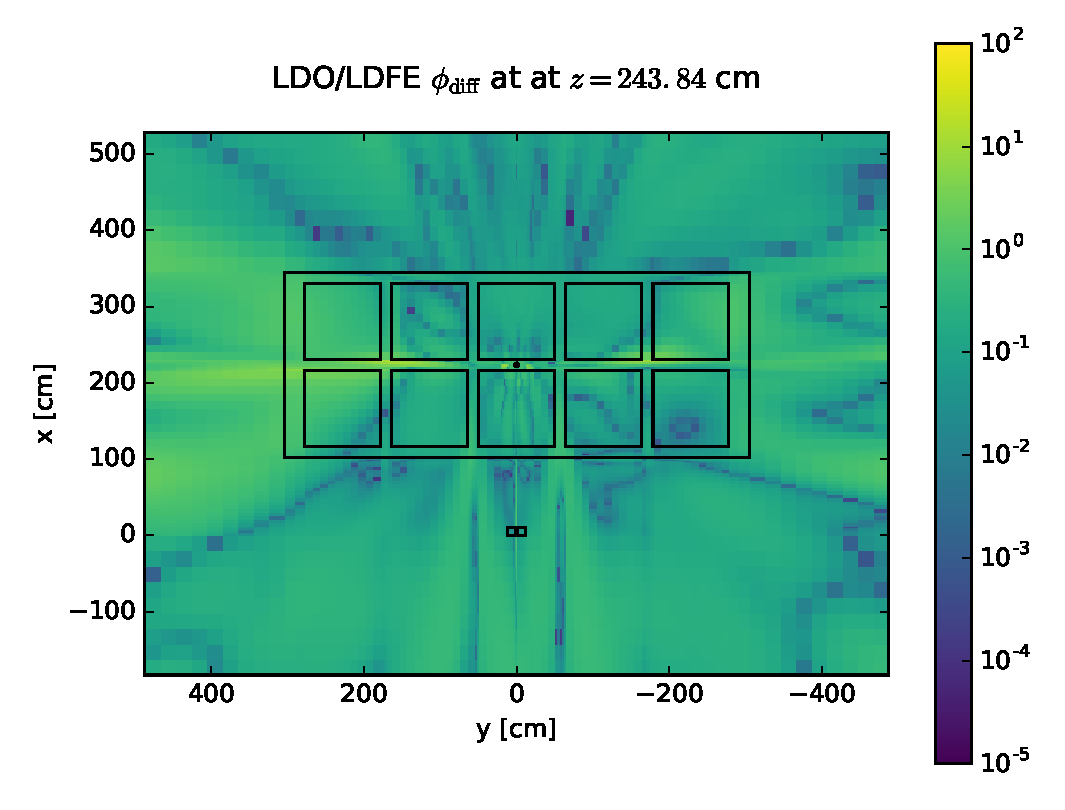
\includegraphics[max height=0.445\textheight]
{img/portal-flux-diff-ldfe.eps}
\subcaption{LDO/LDFE flux relative difference.}
\end{subfigure}
\caption{Simplified portal monitor scenario scalar photon flux relative
         difference slices.}
\label{cargo-fwd-diff-rel}
\end{figure}

\FloatBarrier
%---------------------------------------------------------------------------%%
\subsection{Summary}

For the test cases presented here, we have compared the forward scalar flux solutions
resultant from solving the LDO equations against those arising from solving the
traditional discrete ordinates equations with a small variety of standard
quadrature set types. In
each test case, regardless of particle type, the results from solving the LDO equations best matched those
from using the QR quadrature set in the traditional discrete ordinates
formulation. Additionally, for the benchmark test case, the LDO equations
produced results that best matched the experimental values.

%---------------------------------------------------------------------------%%
\section{Conclusions and Future Work}
\label{sec:conclusions}

In this work, we have seen that the LDO equations' scalar flux solutions are
comparable to those of standard quadrature types. Of particular interest is
the proximity of the LDO solutions to the QR solutions, as QR scalar flux
solutions are commonly used for input in Monte Carlo variance reduction
parameter generation and a future publication will assess the LDO equations'
scalar flux solutions' efficacy as input for Monte Carlo calculation biasing.
The deterministic calculations performed here are an important step towards
that work; we have verified the accuracy of the LDO equations' solutions
relative to those of standard quadrature types.
% Again, this needs to be reframed. The potential use of LDO in general is relevant.
% Focus on the flexibility and their accuracy.
% I'm assuming you're going to add a bit more here? 

\pagebreak
\section*{Acknowledgments}

This material is based upon work supported under an Integrated
University Program Graduate Fellowship as well as supported by the Department 
of Energy under Award Number(s) DE-NE0008661. This report was prepared as an
account of work sponsored by an agency of the United States Government.
Neither the United States Government nor any agency thereof, nor any of their
employees, makes any warranty, express or limited, or assumes any legal
liability or responsibility for the accuracy, completeness, or usefulness of
any information, apparatus, product, or process disclosed, or represents that
its use would not infringe privately owned rights. Reference herein to any 
specific commercial product, process, or service by trade name, trademark, 
manufacturer, or otherwise does not necessarily constitute or imply its 
endorsement, recommendation, or favoring by the United States Government or
any agency thereof. The views and opinions of authors expressed herein do not 
necessarily state or reflect those of the United States Government or any 
agency thereof.

\pagebreak

\bibliographystyle{nse}
\bibliography{ldo-deterministic}

\end{document}
